%=============================================================================
% chktex-file 1 chktex-file 8 chktex-file 12 chktex-file 13 chktex-file 24 chktex-file 26
% RAPPORT DE PROJET DE FIN D'ÉTUDES (PFE) - SESAME
% Titre : LeasRecover - Plateforme SaaS Multi-Tenant pour le Recouvrement
% Auteur : Ilhem Benyedder
%=============================================================================

\documentclass[12pt,a4paper,oneside]{report}

% Configurations and Custom Commands
%=============================================================================
% chktex-file 1 chktex-file 8 chktex-file 12 chktex-file 13 chktex-file 24 chktex-file 26
% PREAMBLE CONFIGURATION - PFE REPORT
%=============================================================================

% Language and Encodings
\usepackage[utf8]{inputenc}
\usepackage[T1]{fontenc}
\usepackage[french]{babel}

% Fonts and Typography
\usepackage{lmodern}
\usepackage{microtype}
\usepackage{setspace}
\onehalfspacing
\setlength{\emergencystretch}{2em}

% Page Geometry
\usepackage[a4paper, top=2.5cm, bottom=2.5cm, left=3cm, right=2.5cm, headheight=15pt]{geometry}
\usepackage{emptypage}

% Colors
\usepackage[table,xcdraw]{xcolor}
\definecolor{primaryblue}{RGB}{24, 76, 120}
\definecolor{secondaryblue}{RGB}{41, 128, 185}
\definecolor{darkslate}{RGB}{44, 62, 80}
\definecolor{accentgreen}{RGB}{39, 174, 96}
\definecolor{accentorange}{RGB}{230, 126, 34}
\definecolor{accentred}{RGB}{192, 57, 43}
\definecolor{lightgrey}{RGB}{245, 247, 250}
\definecolor{bordergrey}{RGB}{220, 224, 230}
\definecolor{codebg}{RGB}{248, 249, 250}

% Mathematics & Symbols
\usepackage{amsmath}
\usepackage{amssymb}
\usepackage{mathtools}

% Algorithms
\usepackage{algorithm}
\usepackage{algorithmic}

% Graphics & TikZ
\usepackage{graphicx}
\usepackage{float}
\usepackage{tikz}
\usetikzlibrary{shapes.geometric, arrows.meta, positioning, shadows, calc, backgrounds, fit, trees}

% Tables
\usepackage{booktabs}
\usepackage{tabularx}
\usepackage{multirow}
\usepackage{colortbl}
\usepackage{array}
\newcolumntype{L}[1]{>{\raggedright\arraybackslash}p{#1}}
\newcolumntype{Y}{>{\raggedright\arraybackslash}X}

% Lists & Formatting
\usepackage{enumitem}
\setlist[itemize]{label=\textbullet, leftmargin=1.5em, itemsep=2pt, parsep=1pt}
\setlist[enumerate]{leftmargin=1.5em, itemsep=2pt, parsep=1pt}

% Code Listings
\usepackage{listings}
\lstdefinestyle{customcode}{
    backgroundcolor=\color{codebg},
    basicstyle=\ttfamily\small,
    breaklines=true,
    breakatwhitespace=true,
    captionpos=b,
    frame=single,
    rulecolor=\color{bordergrey},
    keywordstyle=\color{primaryblue}\bfseries,
    commentstyle=\color{accentgreen}\itshape,
    stringstyle=\color{accentorange},
    numbers=left,
    numberstyle=\tiny\color{darkslate!60},
    stepnumber=1,
    numbersep=8pt,
    tabsize=2,
    showstringspaces=false
}
\lstset{style=customcode}

% Callout Boxes
\usepackage[most]{tcolorbox}
\newtcolorbox{infobox}[2][]{
    enhanced,
    colback=lightgrey,
    colframe=secondaryblue,
    coltitle=white,
    fonttitle=\bfseries\sffamily,
    title={#2},
    arc=3mm,
    boxrule=1pt,
    left=10pt, right=10pt, top=8pt, bottom=8pt,
    #1
}

\newtcolorbox{notebox}[1][]{
    enhanced,
    colback=lightgrey,
    colframe=accentorange,
    arc=2mm,
    boxrule=1pt,
    left=8pt, right=8pt, top=6pt, bottom=6pt,
    #1
}

% Headers and Footers
\usepackage{fancyhdr}
\pagestyle{fancy}
\fancyhf{}
\fancyhead[L]{\small\nouppercase{\leftmark}}
\fancyhead[R]{\small\nouppercase{\rightmark}}
\fancyfoot[C]{\thepage}
\renewcommand{\headrulewidth}{0.5pt}
\renewcommand{\footrulewidth}{0.3pt}

\fancypagestyle{plain}{
    \fancyhf{}
    \fancyfoot[C]{\thepage}
    \renewcommand{\headrulewidth}{0pt}
    \renewcommand{\footrulewidth}{0pt}
}

% Titles & Headings
\usepackage{titlesec}
\titleformat{\chapter}[display]
  {\normalfont\Large\bfseries\color{primaryblue}}
  {\chaptertitlename\ \thechapter}{10pt}{\Huge\bfseries\color{darkslate}}
\titlespacing*{\chapter}{0pt}{-10pt}{25pt}

\titleformat{\section}
  {\normalfont\Large\bfseries\color{primaryblue}\raggedright}
  {\thesection}{1em}{}
\titlespacing*{\section}{0pt}{18pt}{8pt}

\titleformat{\subsection}
  {\normalfont\large\bfseries\color{secondaryblue}\raggedright}
  {\thesubsection}{1em}{}
\titlespacing*{\subsection}{0pt}{12pt}{6pt}

\titleformat{\subsubsection}
  {\normalfont\normalsize\bfseries\color{darkslate}\raggedright}
  {\thesubsubsection}{1em}{}

% Captions
\usepackage[font=small,labelfont={bf,color=primaryblue},format=hang]{caption}
\usepackage{subcaption}
\frenchsetup{SmallCapsFigTabCaptions=false}

% Hyperlinks
\usepackage{hyperref}
\hypersetup{
    colorlinks=true,
    linkcolor=primaryblue,
    citecolor=secondaryblue,
    filecolor=darkslate,
    urlcolor=accentorange,
    pdfauthor={Ilhem Benyedder},
    pdftitle={LeasRecover : Plateforme SaaS Multi-Tenant pour la Digitalisation du Recouvrement et l'Expertise des Véhicules en Leasing},
    pdfsubject={Rapport de Projet de Fin d'Études (PFE)},
    pdfkeywords={Leasing, Recouvrement, SaaS, Multi-Tenant, Expertise Automobile, OCR, FastAPI, React}
}

%=============================================================================
% chktex-file 1 chktex-file 8 chktex-file 12 chktex-file 13 chktex-file 24 chktex-file 26
% CUSTOM COMMANDS AND METADATA - PFE REPORT SESAME
%=============================================================================

% Project Metadata
\newcommand{\projectTitle}{LeasRecover : Plateforme SaaS de Digitalisation du Recouvrement Leasing avec Module d'Intelligence Artificielle pour la Valorisation Automatique des Actifs}
\newcommand{\projectShortTitle}{LeasRecover}
\newcommand{\authorName}{Mlle. Ilhem BEN YEDDER}
\newcommand{\studentClass}{INGTA 4 SE-B}
\newcommand{\academicYear}{2025 -- 2026}
\newcommand{\diploma}{Diplôme d'Ingénieur en Informatique -- Spécialité : Génie Logiciel}
\newcommand{\institution}{SESAME University -- École Supérieure Privée des Sciences Appliquées et de Management}
\newcommand{\hostCompany}{Teamwill Consulting}
\newcommand{\hostCompanyLogo}{images/logo_entreprise.png} % Chemin vers le logo (PNG, JPG, PDF)
\newcommand{\academicAdvisor}{M. Achraf Salmi}
\newcommand{\industrialAdvisor}{M. Hedfi Ahmed}

% Custom Shortcuts
\newcommand{\vr}{\text{VR}} % Valeur Résiduelle
\newcommand{\ve}{\text{VE}} % Valeur d'Expertise
\newcommand{\code}[1]{{\small\texttt{\detokenize{#1}}}}
\newcommand{\req}[1]{\textbf{\textsf{#1}}}

% Acronym helper
\newcommand{\acro}[2]{\textbf{#1} (#2)}


\begin{document}
\hypersetup{pageanchor=false}

%=============================================================================
% PAGE DE GARDE OFFICIELLE (SESAME - Conforme à Page de garde PFE.doc)
%=============================================================================
\begin{titlepage}
\thispagestyle{empty}
\newgeometry{top=0.75cm, bottom=1.27cm, left=1.27cm, right=1.27cm}

% Background subtle polygonal pattern from Page de garde PFE.doc (Full bleed edge-to-edge)
\begin{tikzpicture}[remember picture,overlay]
    \node[inner sep=0pt, outer sep=0pt, anchor=center] at (current page.center) {
        
\includegraphics[width=\paperwidth,height=\paperheight,keepaspectratio=false]{images/cover_pattern.png}
    };
\end{tikzpicture}

\begin{center}

    % SESAME Official Header Banner
    \noindent
\includegraphics[width=\linewidth]{images/sesame_header.png}

    \vspace{1.0cm}

    % Main Title (Calibri Light 18pt Bold Centered)
    {\fontsize{18}{22}\selectfont\bfseries\sffamily RAPPORT DE STAGE DE PROJET DE FIN D'ÉTUDES\par}

    \vspace{0.8cm}

    % Section Intitulé & Auteur (Table 1 from Word doc)
    \noindent\rule{\linewidth}{0.6pt}\\[0.35cm]
    {\fontsize{14}{17}\selectfont\sffamily Intitulé du stage}\\[0.3cm]
    {\fontsize{15}{19}\selectfont\bfseries\sffamily \projectTitle}\\[0.45cm]
    \rule{\linewidth}{0.6pt}\\[0.35cm]
    {\fontsize{14}{17}\selectfont\sffamily Réalisé par}\\[0.3cm]
    {\fontsize{15}{19}\selectfont\bfseries\sffamily \authorName}\\[0.2cm]

    \vspace{0.65cm}

    % Section Entreprise d'accueil avec Logo (Table 2 from Word doc)
    {\fontsize{14}{17}\selectfont\sffamily Entreprise d'accueil}\\[0.25cm]
    \IfFileExists{\hostCompanyLogo}{%
        \includegraphics[height=1.5cm,keepaspectratio]{\hostCompanyLogo}\\[0.2cm]%
    }{%
        {\fontsize{11}{14}\selectfont\itshape\color{black!45}[Logo de l'entreprise]\/}\\[0.15cm]%
    }
    {\fontsize{13}{16}\selectfont\bfseries\sffamily \hostCompany}\\[0.15cm]
    {\color{black!35}\makebox[0.6\linewidth]{\dotfill}}

    \vspace{0.65cm}

    % Section Encadrants (Table 3 from Word doc)
    {\fontsize{14}{17}\selectfont\sffamily Encadrant Entreprise}\\[0.25cm]
    {\fontsize{13}{16}\selectfont\bfseries\sffamily \industrialAdvisor}\\[0.15cm]
    {\color{black!35}\makebox[0.45\linewidth]{\dotfill}}\\[0.45cm]
    {\fontsize{14}{17}\selectfont\sffamily Encadrant SESAME}\\[0.25cm]
    {\fontsize{13}{16}\selectfont\bfseries\sffamily \academicAdvisor}\\[0.15cm]
    {\color{black!35}\makebox[0.45\linewidth]{\dotfill}}

    \vfill

    % Année Universitaire (Footer Box from Word doc)
    {\fontsize{12}{15}\selectfont\bfseries\sffamily Année Universitaire}\\[0.15cm]
    {\fontsize{12}{15}\selectfont\bfseries\sffamily \academicYear}

\end{center}
\restoregeometry
\end{titlepage}
\hypersetup{pageanchor=true}

%=============================================================================
% FRONT MATTER
%=============================================================================
\pagenumbering{roman}
\setcounter{page}{1}

% Dédicaces & Remerciements
%=============================================================================
% REMERCIEMENTS & DÉDICACES
%=============================================================================

\chapter*{Dédicaces}
\addcontentsline{toc}{chapter}{Dédicaces}

\begin{itshape}
\begin{center}
À mes chers parents, pour leurs sacrifices inestimables, leur amour inconditionnel et leur soutien indéfectible.\\
\vspace{0.8cm}
À mes frères et sœurs, pour leurs encouragements continus et leur présence bienveillante.\\
\vspace{0.8cm}
À tous mes enseignants et formateurs, qui ont façonné mon esprit critique et ma passion pour l'ingénierie logicielle.\\
\vspace{0.8cm}
À mes précieux amis et collègues de promotion, avec qui j'ai partagé des moments d'apprentissage inoubliables.\\
\vspace{1.2cm}
\textbf{Ilhem Benyedder}
\end{center}
\end{itshape}

\newpage

\chapter*{Remerciements}
\addcontentsline{toc}{chapter}{Remerciements}

\begin{flushleft}
Je tiens à exprimer ma profonde gratitude et mes sincères remerciements à toutes les personnes qui ont contribué, de près ou de loin, à la réalisation et au succès de ce Projet de Fin d'Études.

J'adresse mes plus vifs remerciements à mon encadrant universitaire, \textbf{\academicAdvisor}, pour sa disponibilité, ses conseils méthodologiques avisés, sa rigueur scientifique et ses orientations précieuses tout au long de l'élaboration de ce travail.

Je remercie chaleureusement mon encadrant industriel, \textbf{\industrialAdvisor}, pour son accompagnement technique constant, ses retours constructifs et sa confiance accordée dans la conception de la solution \projectShortTitle.

Mes sincères remerciements s'adressent également aux membres du jury qui ont accepté d'examiner et d'évaluer ce travail avec bienveillance et rigueur.

Enfin, je remercie l'ensemble du corps professoral et administratif de \textbf{\institution} pour la qualité de l'enseignement dispensé durant tout mon cursus d'ingénieur.
\end{flushleft}


% Résumé & Abstract
%=============================================================================
% chktex-file 1 chktex-file 8 chktex-file 12 chktex-file 13 chktex-file 24 chktex-file 26
% RÉSUMÉ & ABSTRACT
%=============================================================================

\chapter*{Résumé}
\addcontentsline{toc}{chapter}{Résumé}

Le secteur du crédit-bail (\textit{leasing}) financier fait face à des défis opérationnels, juridiques et financiers majeurs lors de la gestion du recouvrement contentieux des véhicules en défaut de paiement. Les processus traditionnels, reposant sur des feuilles de calcul locales disparates et des flux documentaires papier, souffrent de délais de traitement excessifs, d'un manque de traçabilité des échéances légales impératives et d'un risque élevé d'erreurs d'évaluation financière lors de la reprise des actifs sur le marché secondaire.

Ce Projet de Fin d'Études, réalisé au sein de \textbf{\hostCompany}, présente la conception et la réalisation de \textbf{\projectShortTitle}, une plateforme logicielle SaaS (\textit{Software as a Service}) B2B multi-tenant dédiée à l'automatisation intégrale du cycle de recouvrement et d'expertise automobile. La solution structure le workflow réglementaire en cinq phases séquentielles (pré-contentieux, mise en demeure, saisie du véhicule, vente et clôture), tout en intégrant un pipeline d'intelligence artificielle asynchrone capable d'extraire automatiquement les données financières des rapports d'expertise PDF non structurés (NLP/LLM) et de confronter instantanément la valeur marchande réelle à la valeur résiduelle contractuelle.

Développée avec une architecture microservices polyglotte moderne associant \textbf{Next.js 16} (BFF sécurisé), \textbf{Spring Boot 4} (Java 21), \textbf{FastAPI} (Python 3.11), \textbf{PostgreSQL 18} avec isolation multi-tenant par schémas étanches et \textbf{Docker}, la plateforme garantit une conformité légale rigoureuse (RGPD / Loi n°63-2004), une traçabilité d'audit immuable et une réduction substantielle des pertes financières pour les institutions de crédit-bail.

\vspace{0.8cm}
\noindent\textbf{Mots-clés :} Crédit-bail automobile, Recouvrement contentieux, SaaS Multi-Tenant, Intelligence Artificielle, LLM, NLP, Next.js, Spring Boot, FastAPI, PostgreSQL.

\newpage

\chapter*{Abstract}
\addcontentsline{toc}{chapter}{Abstract}

The automotive leasing industry faces critical operational, regulatory, and financial challenges in managing debt collection and asset repossession for defaulted contracts. Traditional management workflows, heavily reliant on fragmented spreadsheets, manual paper trails, and unindexed PDF reports, suffer from severe administrative delays, lack of statutory deadline tracking, and significant inaccuracies during asset remarketing.

This graduation thesis, conducted at \textbf{\hostCompany}, introduces \textbf{\projectShortTitle}, an enterprise B2B multi-tenant SaaS (\textit{Software as a Service}) platform designed to digitize and automate the entire vehicle recovery and appraisal lifecycle. The system enforces a strict 5-phase regulatory workflow (pre-litigation, formal notice, vehicle seizure, asset remarketing, and case closure). At its core, an asynchronous AI-powered document intelligence pipeline leverages NLP and Large Language Models (LLMs) to parse unstructured appraisal PDF reports, automatically benchmarking real-time market value against contractual residual value.

Built with a modern polyglot microservices architecture combining \textbf{Next.js 16} (secure BFF layer with HttpOnly cookies), \textbf{Spring Boot 4} (Java 21), \textbf{FastAPI} (Python 3.11), \textbf{PostgreSQL 18} (schema-per-tenant isolation), and \textbf{Docker}, the platform guarantees absolute data confidentiality, immutable audit logging, regulatory compliance (GDPR / Law No. 63-2004), and measurable financial risk reduction.

\vspace{0.8cm}
\noindent\textbf{Keywords :} Automotive Leasing, Debt Recovery, Multi-Tenant SaaS, Artificial Intelligence, LLM, NLP, Document Understanding, Next.js, Spring Boot, FastAPI, PostgreSQL.


% Tables des matières, figures et tableaux
\tableofcontents
\newpage
\listoffigures
\newpage
\listoftables
\newpage

% Liste des Acronymes et Abréviations
\chapter*{Liste des Abréviations}
\addcontentsline{toc}{chapter}{Liste des Abréviations}

\noindent\begin{tabularx}{\textwidth}{@{}l Y@{}}
\toprule
\textbf{Acronyme} & \textbf{Signification} \\
\midrule
\textbf{PFE} & Projet de Fin d'Études \\
\textbf{SaaS} & Software as a Service \\
\textbf{API} & Application Programming Interface \\
\textbf{REST} & Representational State Transfer \\
\textbf{JWT} & JSON Web Token \\
\textbf{RBAC} & Role-Based Access Control \\
\textbf{RLS} & Row-Level Security \\
\textbf{ORM} & Object-Relational Mapping \\
\textbf{MCD} & Modèle Conceptuel des Données \\
\textbf{MLD} & Modèle Logique des Données \\
\textbf{UML} & Unified Modeling Language \\
\textbf{OCR} & Optical Character Recognition \\
\textbf{NLP} & Natural Language Processing \\
\textbf{VIN} & Vehicle Identification Number (Numéro de châssis) \\
\textbf{$\vr$} & Valeur Résiduelle contractuelle \\
\textbf{$\ve$} & Valeur d'Expertise marchande \\
\textbf{ACID} & Atomicité, Cohérence, Isolation, Durabilité \\
\bottomrule
\end{tabularx}

\newpage

%=============================================================================
% MAIN MATTER
%=============================================================================
\pagenumbering{arabic}
\setcounter{page}{1}

% Introduction Générale
%=============================================================================
% chktex-file 1 chktex-file 8 chktex-file 12 chktex-file 13 chktex-file 24 chktex-file 26
% INTRODUCTION GÉNÉRALE
%=============================================================================

\chapter*{Introduction Générale}
\addcontentsline{toc}{chapter}{Introduction Générale}
\markboth{Introduction Générale}{Introduction Générale}

\section*{Contexte et Enjeux Métiers}

Le secteur du crédit-bail financier (\textit{leasing}) joue un rôle indispensable dans le financement des investissements des entreprises et des ménages, leur permettant d'acquérir des actifs matériels et des parcs automobiles sans impacter massivement leur trésorerie courante. Néanmoins, la gestion des risques de défaut de paiement représente un défi opérationnel et réglementaire permanent pour les institutions de crédit et les bailleurs. En effet, dès lors qu'un locataire entre en situation d'impayé persistant, un engrenage juridique, logistique et financier complexe se met en branle, allant des relances amiables initiales jusqu'à la saisie conservatoire et la revente forcée de l'actif gagé.

\section*{État des Lieux et Problématique}

Actuellement, ce processus de recouvrement souffre d'une fragmentation logicielle critique au sein de nombreuses sociétés de leasing. Les gestionnaires opérationnels se retrouvent contraints d'orchestrer ces procédures via un assemblage hétérogène de feuilles de calcul Excel locales, de courriers papier et de systèmes d'archivage non interconnectés. Cette absence de centralisation engendre deux risques majeurs :
\begin{itemize}
    \item \textbf{Un risque de perte financière directe :} L'évaluation approximative ou tardive des actifs repris sur le marché secondaire fausse les prix de mise en vente et le calibrage des provisions comptables. Le traitement manuel des rapports d'expertise de véhicules (fichiers PDF non structurés) requiert entre 30 et 60 minutes par dossier, ralentissant considérablement la réactivité des équipes.
    \item \textbf{Un risque juridique majeur :} En phase pré-contentieuse et judiciaire, l'omission ou le retard dans l'envoi d'une pièce légale (telle qu'une mise en demeure officielle ou une sommation de payer) peut vicier la procédure et provoquer son invalidation totale devant les tribunaux, en vertu des délais légaux stricts imposés par les réglementations nationales et internationales (notamment le RGPD en Europe et la Loi organique n°63-2004 en Tunisie).
\end{itemize}

Face à ce double défi, la problématique centrale de notre travail s'énonce ainsi :

\begin{quote}
\textit{« Comment concevoir et développer une plateforme logicielle SaaS multi-tenant, sécurisée et intégrable, capable d'automatiser l'intégralité du workflow de recouvrement leasing en garantissant le respect strict des délais légaux, tout en exploitant un pipeline d'intelligence artificielle pour optimiser la valorisation financière des actifs repris ? »}
\end{quote}

\section*{Proposition de Solution : La Plateforme \projectShortTitle}

C'est dans ce contexte que s'inscrit le projet \textbf{\projectShortTitle}, conçu et réalisé au sein de \textbf{\hostCompany}. \projectShortTitle{} est une plateforme SaaS (\textit{Software as a Service}) B2B multi-tenant dont l'ambition est de digitaliser intégralement le cycle de vie du recouvrement leasing autour de quatre piliers fondamentaux :
\begin{enumerate}
    \item \textbf{Workflow Réglementaire Strict :} Automatisation et sécurisation du cycle de vie des dossiers à travers cinq phases séquentielles rigoureusement encadrées (Pré-contentieux $\rightarrow$ Mise en demeure $\rightarrow$ Saisie du véhicule $\rightarrow$ Vente $\rightarrow$ Clôture).
    \item \textbf{Pipeline d'Extraction par Intelligence Artificielle :} Un microservice asynchrone s'appuyant sur des modèles de Traitement Automatique du Langage Naturel (NLP) et de grands modèles de langage (LLM) pour analyser les rapports d'expertise, extraire les caractéristiques du véhicule et confronter instantanément la valeur marchande réelle ($\ve$) à la valeur résiduelle comptable ($\vr$).
    \item \textbf{Moteur d'Alertes et de Pilotage Proactif :} Suivi en temps réel des délais juridiques et détection automatique des dossiers stagnants ou dormants afin de prévenir toute péremption légale.
    \item \textbf{Isolation SaaS Hermétique et Traçabilité Réglementaire :} Implémentation d'une architecture multi-tenant assurant l'étanchéité absolue des données entre entreprises clientes, couplée à un journal d'audit (\textit{Audit Trail}) immuable.
\end{enumerate}

\section*{Organisation du Rapport}

Le présent document retrace l'ensemble des étapes de recherche, de modélisation, d'architecture et de réalisation de la plateforme \projectShortTitle. Il est articulé autour de quatre chapitres fondamentaux :
\begin{itemize}
    \item \textbf{Chapitre 1 -- Contexte Général du Projet et État de l'Art :} Présente l'organisme d'accueil \hostCompany, dresse l'étude critique de l'existant, examine l'état de l'art technologique et expose la démarche agile retenue.
    \item \textbf{Chapitre 2 -- Spécification et Analyse des Besoins :} Formalise les exigences fonctionnelles et non-fonctionnelles, identifie les acteurs, présente la modélisation UML (diagrammes de cas d'utilisation par module, diagramme de classes), la planification par sprints et l'architecture logique globale.
    \item \textbf{Chapitre 3 -- Conception Architecturale et Détaillée :} Approfondit le modèle conceptuel de données (MCD), la stratégie d'isolation multi-tenant, la spécification détaillée des cas d'utilisation (UC1 à UC4) et la formulation du moteur d'arbitrage financier.
    \item \textbf{Chapitre 4 -- Réalisation, Pipeline IA et Validation :} Décrit l'environnement technologique de production, le fonctionnement du pipeline d'extraction IA, les interfaces utilisateurs clés et la campagne de tests et validation.
\end{itemize}


% Chapitres
%=============================================================================
% chktex-file 1 chktex-file 8 chktex-file 12 chktex-file 13 chktex-file 24 chktex-file 26
% CHAPITRE 1 : CONTEXTE GÉNÉRAL DU PROJET ET ÉTAT DE L'ART
%=============================================================================

\chapter{Contexte Général du Projet et État de l'Art}
\label{chap:contexte}

\section{Introduction}

Ce chapitre présente le contexte global du projet \textbf{\projectShortTitle}. Il décrit d'abord l'organisme d'accueil \textbf{\hostCompany}, dresse un état des lieux critique des processus de recouvrement actuels au sein des sociétés de leasing, examine l'état de l'art des solutions technologiques disponibles, et détaille enfin la problématique à laquelle notre plateforme SaaS se propose d'apporter une réponse moderne, sécurisée et pérenne.

\section{Présentation de l'Organisme d'Accueil et Contexte du Stage}

\subsection{Présentation de l'Entreprise Teamwill Consulting}

Le projet a été développé au sein de \textbf{\hostCompany}. L'entreprise s'impose comme un leader international incontournable du conseil et de l'intégration de solutions logicielles spécifiquement dédiées aux métiers du crédit et du leasing financier. Acteur technologique de référence du secteur Fintech, Teamwill accompagne les banques, les institutions financières et les bailleurs spécialisés dans la refonte de leurs architectures métiers et la transformation numérique de leurs activités.

\subsection{Contexte du Stage}

Ce projet s'inscrit dans le cadre de mon Projet de Fin d'Études d'ingénieur d'une durée réglementaire de six mois. L'objectif assigné par \hostCompany\ consiste à concevoir et à implémenter la plateforme \projectShortTitle. Ce stage permet d'allier la digitalisation de processus juridiques et financiers complexes à la mise en œuvre de technologies avancées, notamment le développement d'une architecture microservices multi-tenant et l'intégration de modules d'intelligence artificielle (LLM/NLP).

\section{Étude et Critique de l'Existant}

\subsection{Analyse de l'Existant}

Actuellement, les départements de recouvrement des sociétés de leasing opèrent dans un environnement caractérisé par une forte fragmentation des outils numériques. Les processus opérationnels s'organisent principalement autour de fichiers tableurs Excel locaux, d'échanges d'e-mails manuels et de dossiers physiques au format papier.

Cette rupture technologique devient critique lors de la phase de saisie et de valorisation des actifs. Lorsqu'un expert automobile transmet son rapport d'évaluation pour un véhicule repris, ce document se présente sous la forme d'un fichier PDF textuel non structuré. Les informations capitales (caractéristiques mécaniques, kilométrage réel, état général, estimation financière) doivent être extraites manuellement par le gestionnaire de recouvrement. Cette manipulation fastidieuse requiert entre 30 et 60 minutes de travail administratif par dossier, ralentissant considérablement la réactivité opérationnelle des équipes.

\subsection{Critique de l'Existant}

L'analyse approfondie du système traditionnel met en relief trois dysfonctionnements majeurs :
\begin{itemize}
    \item \textbf{Dysfonctionnement Organisationnel :} L'absence de centralisation engendre une opacité sur l'état d'avancement des portefeuilles de créances en souffrance. Les gestionnaires manquent d'une visibilité en temps réel pour hiérarchiser efficacement leurs actions et suivre les jalons des dossiers.
    \item \textbf{Dysfonctionnement Financier :} L'évaluation approximative ou tardive des actifs repris sur le marché secondaire provoque des erreurs d'appréciation. Des véhicules mal évalués entraînent des prix de mise en vente inadéquats, des provisions comptables mal calibrées et des pertes financières directes lors de la liquidation de l'actif.
    \item \textbf{Dysfonctionnement Réglementaire et Risques :} En phase pré-contentieuse et contentieuse, l'omission ou le retard dans l'envoi d'une pièce légale (telle qu'une mise en demeure officielle) peut vicier la procédure et provoquer son invalidation totale devant les tribunaux. Les outils actuels n'offrent aucun mécanisme de contrôle ou d'alerte automatisé face à ces délais légaux impératifs (notamment en conformité avec le RGPD et la Loi organique n°63-2004).
\end{itemize}

\begin{table}[H]
\centering
\small
\caption{Comparaison synthétique entre le processus existant et la solution \projectShortTitle}
\label{tab:comparaison_existant}
\begin{tabularx}{\textwidth}{@{}L{3.1cm} L{5.5cm} Y@{}}
\toprule
\textbf{Dimension} & \textbf{Processus Traditionnel (Existant)} & \textbf{Plateforme \projectShortTitle} \\
\midrule
\textbf{Support de gestion} & Feuilles Excel locales et dossiers papier dispersés. & Base de données PostgreSQL centralisée en architecture SaaS. \\
\addlinespace
\textbf{Gestion des délais} & Rappels manuels sur agenda, risque élevé d'omission. & Moteur d'alertes proactif et calcul des échéances légales en temps réel. \\
\addlinespace
\textbf{Traitement de l'expertise} & Saisie manuelle lente (30 à 60 min) depuis des PDF scans. & Extraction asynchrone par IA (NLP/LLM) en moins de 30 secondes. \\
\addlinespace
\textbf{Arbitrage financier} & Comparaison $\ve$ vs $\vr$ manuelle et intuitive. & Calcul automatisé de l'écart $\Delta = |\ve - \vr|$ avec indicateur de fiabilité. \\
\addlinespace
\textbf{Traçabilité \& Audit} & Absence d'historique consolidé et vérifiable. & Journal d'audit (\textit{Audit Trail}) immuable pour chaque mutation. \\
\addlinespace
\textbf{Sécurité des données} & Fichiers circulant sans chiffrement. & Chiffrement AES-256 / TLS, isolation multi-tenant stricte. \\
\bottomrule
\end{tabularx}
\end{table}

\section{État de l'Art Technologique}

Sur le marché des technologies financières, les progiciels de leasing classiques (LMS/ERP) gèrent de manière efficace la phase active des contrats et la facturation courante, mais s'arrêtent dès que survient le défaut de paiement persistant. À l'inverse, les logiciels de recouvrement génériques n'intègrent pas les spécificités des workflows réglementaires du leasing, ni la gestion physique et financière des actifs automobiles saisis.

Par ailleurs, si les technologies d'OCR (\textit{Optical Character Recognition}) traditionnelles parviennent à numériser du texte brut, elles s'avèrent incapables d'en comprendre le contexte sémantique. L'application combinée de modèles de langage (LLM) et de traitement automatique du langage naturel (NLP) pour analyser un rapport d'expertise complexe et le confronter automatiquement à la valeur résiduelle comptable d'un contrat constitue une approche originale absente des solutions logicielles actuelles.

\section{Problématique et Démarche Adoptée}

\subsection{Présentation de la Problématique}

L'écart de performance constaté entre les exigences de conformité juridico-financières et la réalité des traitements manuels nous amène à formaliser la problématique suivante :

\begin{quote}
\textit{« Comment concevoir et développer une plateforme logicielle SaaS multi-tenant, sécurisée et intégrable, capable d'automatiser l'intégralité du workflow de recouvrement leasing en garantissant le respect strict des délais légaux nationaux et internationaux, tout en exploitant un pipeline d'intelligence artificielle pour optimiser la valorisation financière des actifs repris ? »}
\end{quote}

\subsection{Proposition de Solution : LeasRecover}

Pour résoudre cette problématique, la plateforme \projectShortTitle\ a été structurée autour de quatre piliers fondamentaux :
\begin{enumerate}
    \item \textbf{Workflow Réglementaire Strict :} Automatisation et sécurisation du cycle de vie des dossiers à travers 5 phases séquentielles (Pré-contentieux $\rightarrow$ Mise en demeure $\rightarrow$ Saisie du véhicule $\rightarrow$ Vente $\rightarrow$ Clôture).
    \item \textbf{Pipeline d'Extraction par IA :} Un microservice asynchrone (FastAPI/Python) s'appuyant sur des modèles LLM/NLP pour analyser les rapports d'expertise, extraire les caractéristiques du véhicule, calculer la déviation financière face à la valeur résiduelle initiale et générer un indicateur de fiabilité tripartite.
    \item \textbf{Moteur d'Alertes Proactif :} Suivi en temps réel des délais juridiques et détection automatique des dossiers stagnants ou dormants afin de prévenir toute péremption légale.
    \item \textbf{Isolation SaaS et Traçabilité :} Implémentation d'un modèle multi-tenant garantissant l'étanchéité absolue des données entre entreprises clientes, couplée à un historique d'Audit Trail immuable pour répondre aux exigences de preuve juridique (RGPD / Loi n°63-2004).
\end{enumerate}

\subsection{Démarche Méthodologique Adoptée}

La réalisation de ce projet industriel en tant que développeur unique a imposé l'adoption d'une démarche itérative Agile inspirée du framework \textbf{Scrum}. Le cycle de développement a été planifié selon une logique d'incréments fonctionnels précis :
\begin{itemize}
    \item \textbf{Incrément 1 (Fondations \& Sécurité) :} Initialisation de l'infrastructure multi-tenant (schémas PostgreSQL isolés), sécurisation des API via un pattern Backend-For-Frontend (BFF) avec cookies HttpOnly et gestion de l'identité.
    \item \textbf{Incrément 2 (Cœur Métier \& Workflow) :} Modélisation des entités métiers (Clients, Contrats, Véhicules), gestion des dossiers contentieux et mise en œuvre du moteur de transitions d'états conditionnel.
    \item \textbf{Incrément 3 (IA \& Intelligence Documentaire) :} Développement du service Python FastAPI pour l'analyse documentaire, interconnexion asynchrone par webhooks et routage des alertes sur le tableau de bord du gestionnaire.
\end{itemize}

\section{Conclusion}

Ce premier chapitre a posé le cadre de référence du projet \projectShortTitle\ au sein de \hostCompany. L'étude critique de l'existant a mis en évidence la nécessité impérieuse de rompre avec les processus manuels générateurs de risques et de pertes financières. Le chapitre suivant se focalisera sur la spécification détaillée et l'analyse approfondie des besoins fonctionnels et techniques indispensables à la réussite de la plateforme.

%=============================================================================
% chktex-file 1 chktex-file 8 chktex-file 12 chktex-file 13 chktex-file 24 chktex-file 26
% CHAPITRE 2 : SPÉCIFICATION ET ANALYSE DES BESOINS
%=============================================================================

\chapter{Spécification et Analyse des Besoins}
\label{chap:besoins}

\section{Introduction}

L'analyse des besoins s'appuie sur l'étude approfondie du processus de recouvrement dans le secteur du crédit-bail financier. Ce chapitre se décompose en plusieurs sections fondamentales : la définition du langage de modélisation et de la méthodologie adoptée, la spécification détaillée des exigences fonctionnelles et non fonctionnelles, l'analyse par la modélisation UML (diagrammes de cas d'utilisation par module et diagramme de classes), la planification des sprints, et enfin la présentation des architectures logique et physique du système ainsi que l'étude des outils technologiques.

\section{Langage de Modélisation et Méthodologie}

\subsection{Langage de Modélisation : UML}

Le langage \textbf{UML} (\textit{Unified Modeling Language}) est utilisé comme méthode standardisée de modélisation et de visualisation. Il facilite la conception orientée objet en décrivant formellement les interactions dynamiques du système (diagramme de cas d'utilisation) et sa structure statique (diagramme de classes).

\subsection{Méthodologie Adoptée : Scrum}

Pour mener à bien la conception et le développement de la plateforme \projectShortTitle, le framework Agile \textbf{Scrum} a été retenu. Il permet une livraison itérative et incrémentale. Face à la complexité d'une architecture multi-tenant et d'un pipeline d'intelligence artificielle, Scrum offre une transparence et une visibilité accrues sur l'avancement. Des sprints réguliers permettent de valider les fonctionnalités critiques telles que l'isolation des données ou l'extraction documentaire, tout en s'adaptant continuellement aux retours et aux enjeux d'intégration.

\section{Spécification des Besoins}

\subsection{Identification des Acteurs}

Le système interagit avec plusieurs acteurs présentant des responsabilités fonctionnelles distinctes :
\begin{itemize}
    \item \textbf{Super Admin (Éditeur LeasRecover) :} Crée, configure et supervise les \textit{tenants} (sociétés de leasing clientes). Il n'a aucun accès aux données contenues dans les dossiers clients de ses locataires.
    \item \textbf{Admin (Société cliente) :} Configure l'environnement spécifique à son tenant (image de marque, délais légaux par phase, seuils d'alerte IA) et gère les comptes de ses Gestionnaires.
    \item \textbf{Gestionnaire de Recouvrement :} Utilisateur opérationnel final. Il crée les dossiers, pilote le workflow en 5 phases, téléverse les rapports d'expertise et prend les décisions d'arbitrage de vente.
    \item \textbf{Module IA (Acteur Système) :} Composant automatisé qui analyse les rapports d'expertise de manière asynchrone, extrait les valeurs financières clés et calcule l'écart avec la valeur résiduelle initiale.
\end{itemize}

\subsection{Besoins Fonctionnels}

Les fonctionnalités attendues sont organisées en trois modules logiques principaux :

\subsubsection{Module 1 : Administration et Gestion des Tenants}
\begin{itemize}
    \item Création, activation, suspension et isolation stricte des tenants (sociétés de leasing).
    \item Configuration personnalisée des délais légaux par phase et des seuils d'inactivité/dormance.
    \item Gestion granulaire des utilisateurs et des permissions associées aux rôles au sein du tenant.
\end{itemize}

\subsubsection{Module 2 : Cœur Métier (Dossiers et Workflow)}
\begin{itemize}
    \item Création et suivi des dossiers de recouvrement rattachés à un client débiteur, un contrat de leasing et un véhicule.
    \item Progression conditionnelle via 5 phases séquentielles : \textbf{Pré-contentieux} $\rightarrow$ \textbf{Mise en demeure} $\rightarrow$ \textbf{Saisie} $\rightarrow$ \textbf{Vente} $\rightarrow$ \textbf{Clôture}.
    \item Génération automatique d'alertes à l'approche de l'expiration d'un délai légal ou d'un seuil d'inactivité critique.
    \item Coffre-fort documentaire sécurisé pour le stockage des pièces juridiques.
\end{itemize}

\subsubsection{Module 3 : Intelligence Artificielle et Évaluation Documentaire}
\begin{itemize}
    \item Téléversement sécurisé de rapports d'expertise PDF et déclenchement automatique du pipeline asynchrone IA.
    \item Extraction sémantique de la valeur marchande ($\ve$) et confrontation instantanée à la valeur résiduelle contractuelle ($\vr$).
    \item Génération d'un indicateur de fiabilité financière explicite (\textit{Fiable}, \textit{Écart modéré}, \textit{Écart critique}).
\end{itemize}

\subsection{Besoins Non Fonctionnels}

Les exigences non fonctionnelles garantissent la robustesse et l'opérabilité de la plateforme B2B :
\begin{itemize}
    \item \textbf{Performance :} Le pipeline IA complet doit s'exécuter en moins de 30 secondes par rapport d'expertise. Le tableau de bord principal doit se charger en moins de 2 secondes.
    \item \textbf{Sécurité et Confidentialité :} Chiffrement de niveau industriel (AES-256 au repos, TLS 1.2+ en transit) et isolation multi-tenant à tolérance zéro assurée au niveau de la base de données.
    \item \textbf{Traçabilité \& Conformité :} Enregistrement automatique de chaque action utilisateur dans un journal d'audit (\textit{Audit Trail}) immuable, garantissant la conformité avec le RGPD et la Loi n°63-2004.
    \item \textbf{Scalabilité \& Disponibilité :} Le microservice IA doit être déployé et mis à l'échelle indépendamment du reste de l'application métier.
\end{itemize}

\section{Analyse des Besoins}

\subsection{Diagrammes des Cas d'Utilisation}

Afin de garantir une lisibilité optimale et une modélisation rigoureuse des interactions, les cas d'utilisation de la plateforme \projectShortTitle{} sont découpés en quatre diagrammes modulaires correspondant aux grands packages fonctionnels et aux rôles des acteurs.

\subsubsection{Cas d'Utilisation 1 : Administration des Tenants et Politiques de Conformité}

Ce premier module (figure~\ref{fig:uc1_admin_compliance}) modélise l'espace d'administration de la plateforme, partagé entre le Super Administrateur (éditeur de la solution) et l'Administrateur de l'organisme de leasing :

\begin{figure}[H]
\centering
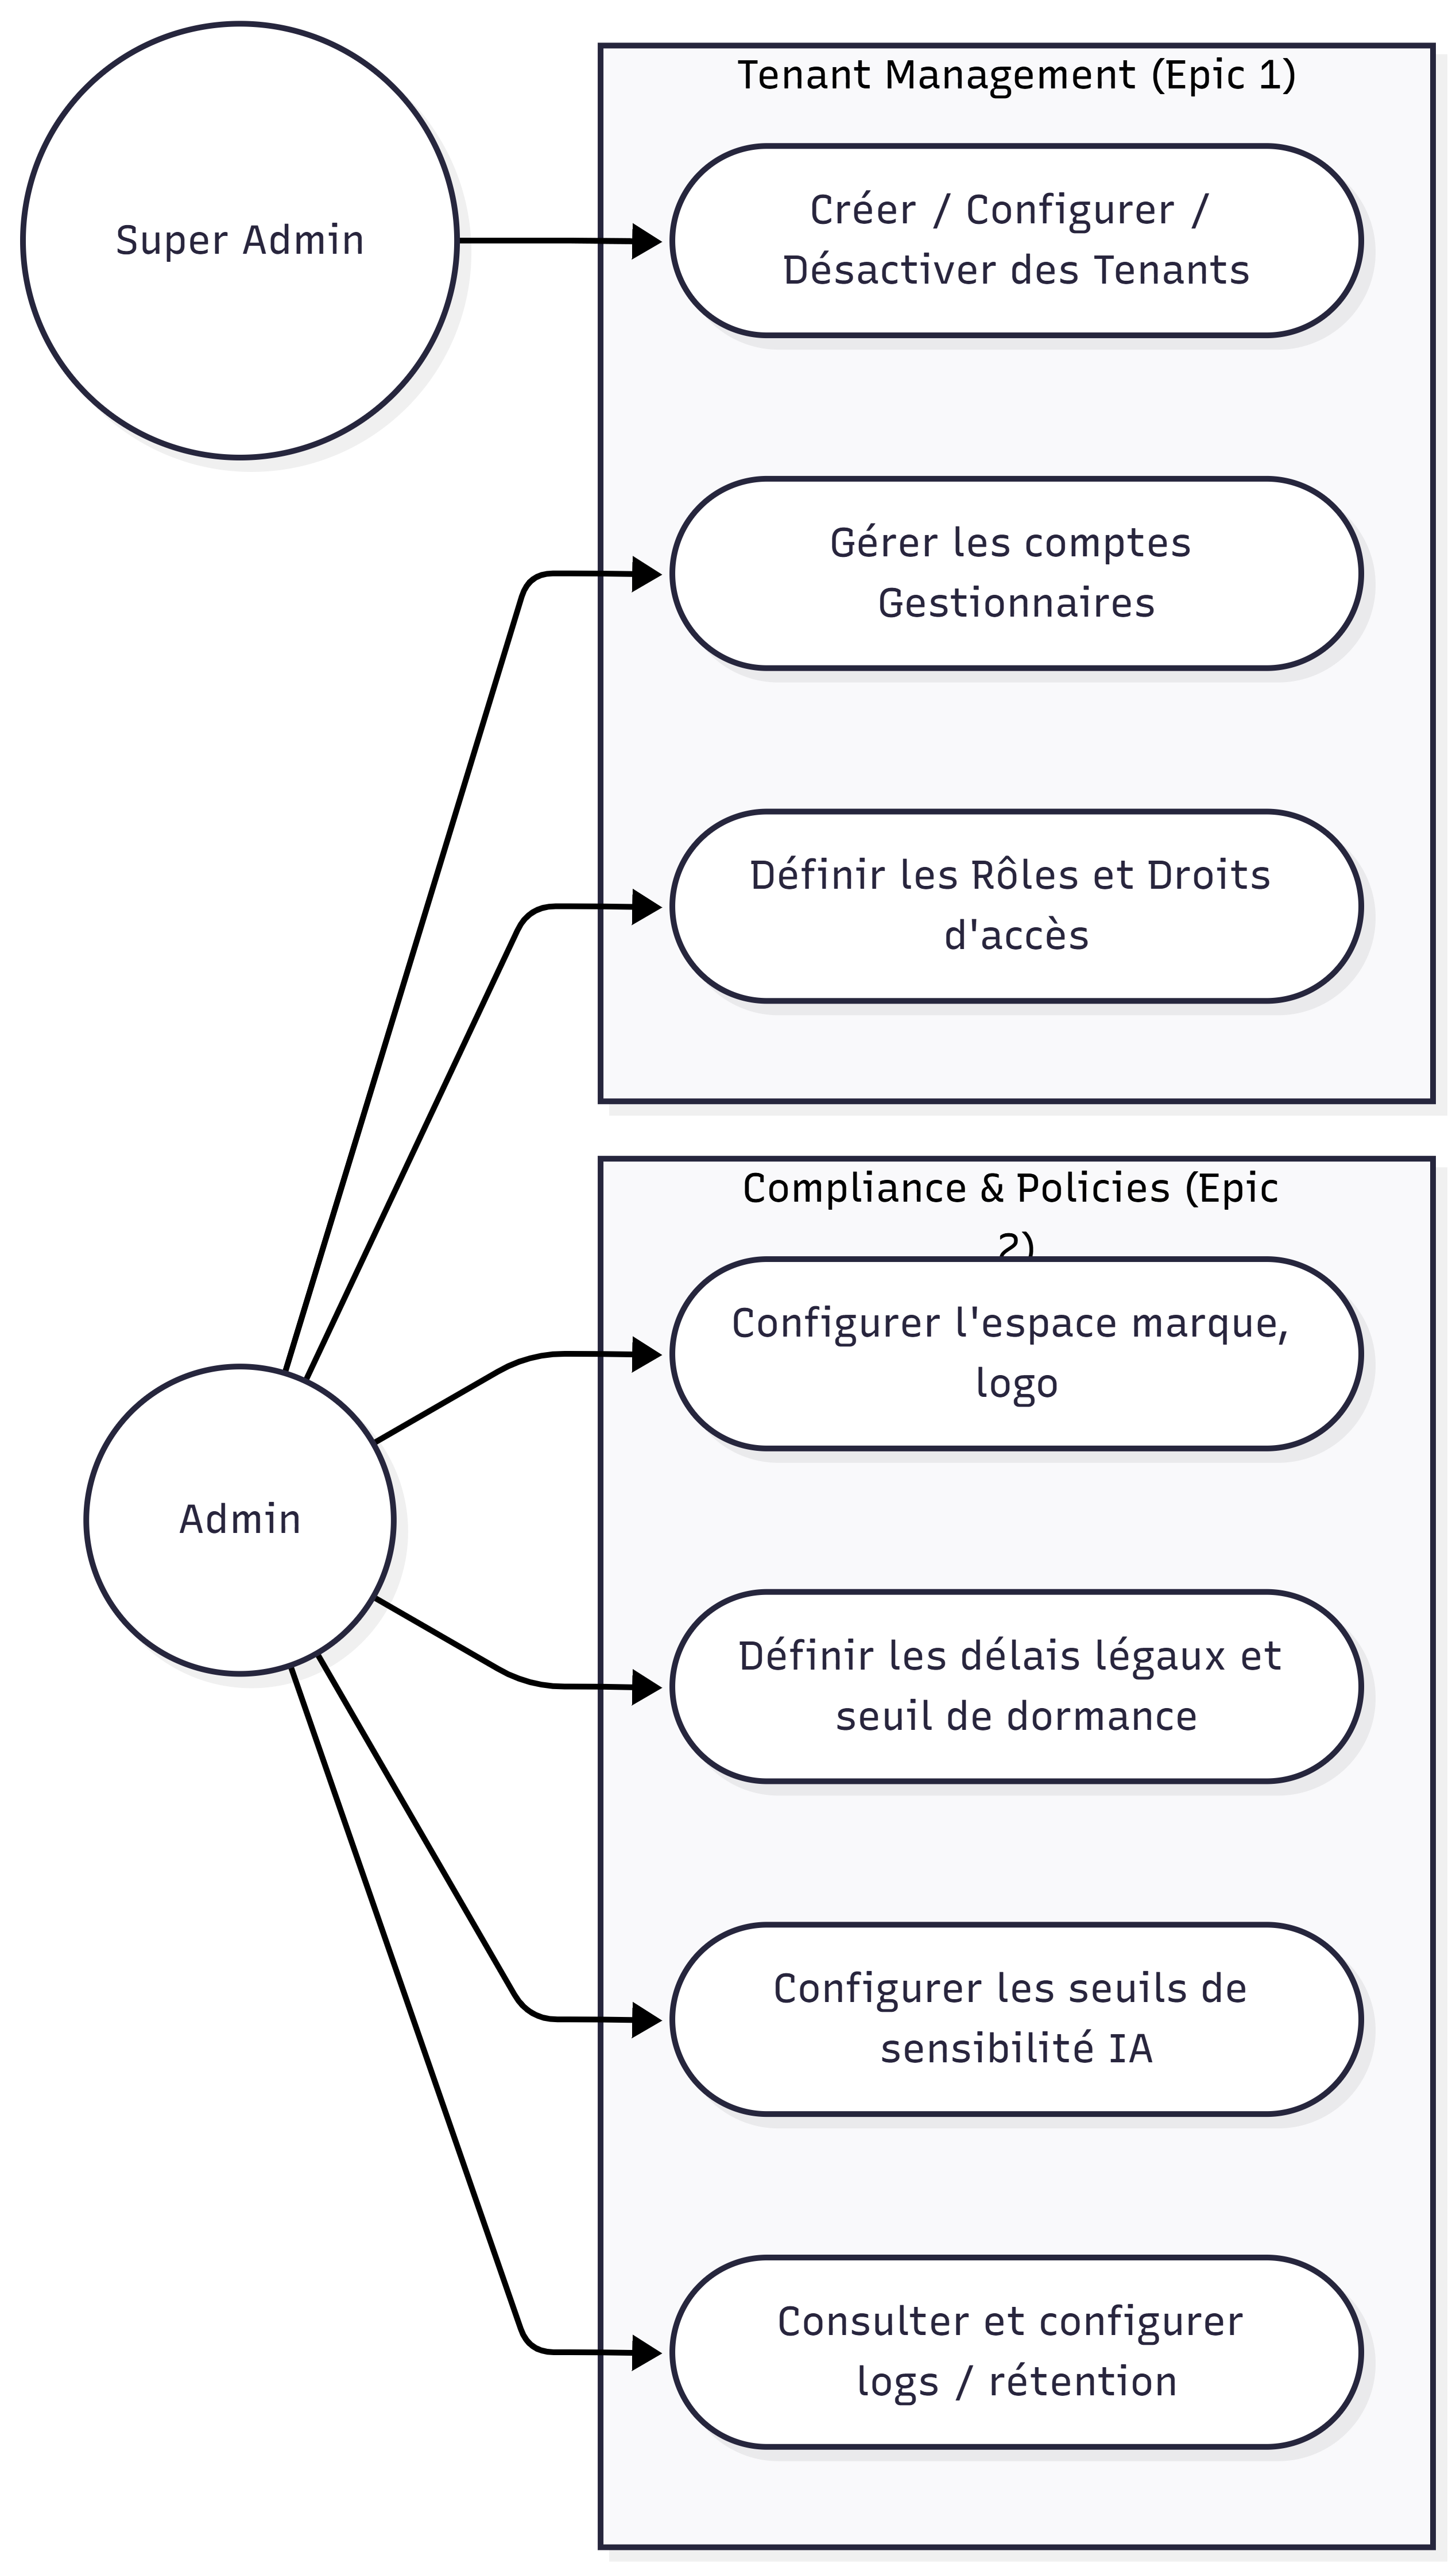
\includegraphics[width=\textwidth,height=0.62\textheight,keepaspectratio]{images/uc1.png}
\caption{Diagramme de cas d'utilisation -- Administration des Tenants et Conformité}
\label{fig:uc1_admin_compliance}
\end{figure}

\begin{itemize}
    \item \textbf{Super Administrateur (Éditeur LeasRecover) :}
    \begin{itemize}
        \item \textit{Créer, Configurer et Désactiver des Tenants :} Provisionnement sécurisé d'une nouvelle société cliente, instanciation automatique de son schéma de données étanche et gestion de l'état d'activité de l'instance.
    \end{itemize}
    \item \textbf{Administrateur (Société de leasing cliente) :}
    \begin{itemize}
        \item \textit{Gestion des comptes gestionnaires :} Création, affectation et révocation des accès des gestionnaires de recouvrement.
        \item \textit{Définition des rôles et privilèges :} Attribution granulaire des droits d'accès (RBAC) sur les dossiers et actions financières.
        \item \textit{Personnalisation de la marque (Tenant Branding) :} Téléversement du logo institutionnel et personnalisation visuelle de l'espace de travail.
        \item \textit{Paramétrage des délais légaux et seuil de dormance :} Définition des délais légaux maximaux par phase et du seuil d'inactivité déclenchant la qualification de dossier dormant.
        \item \textit{Configuration des seuils de sensibilité IA :} Définition des pourcentages d'écart de valeur déclenchant les alertes de dépréciation.
        \item \textit{Consultation des logs et politiques de rétention :} Traçabilité des actions administratives et configuration des durées de conservation des journaux d'audit.
    \end{itemize}
\end{itemize}

\subsubsection{Cas d'Utilisation 2 : Gestion des Référentiels Métiers et Dossiers de Recouvrement}

Le deuxième module (figure~\ref{fig:uc2_core_cases}) détaille la gestion du référentiel métier ainsi que le cycle de vie opérationnel des dossiers de recouvrement contentieux :

\begin{figure}[H]
\centering
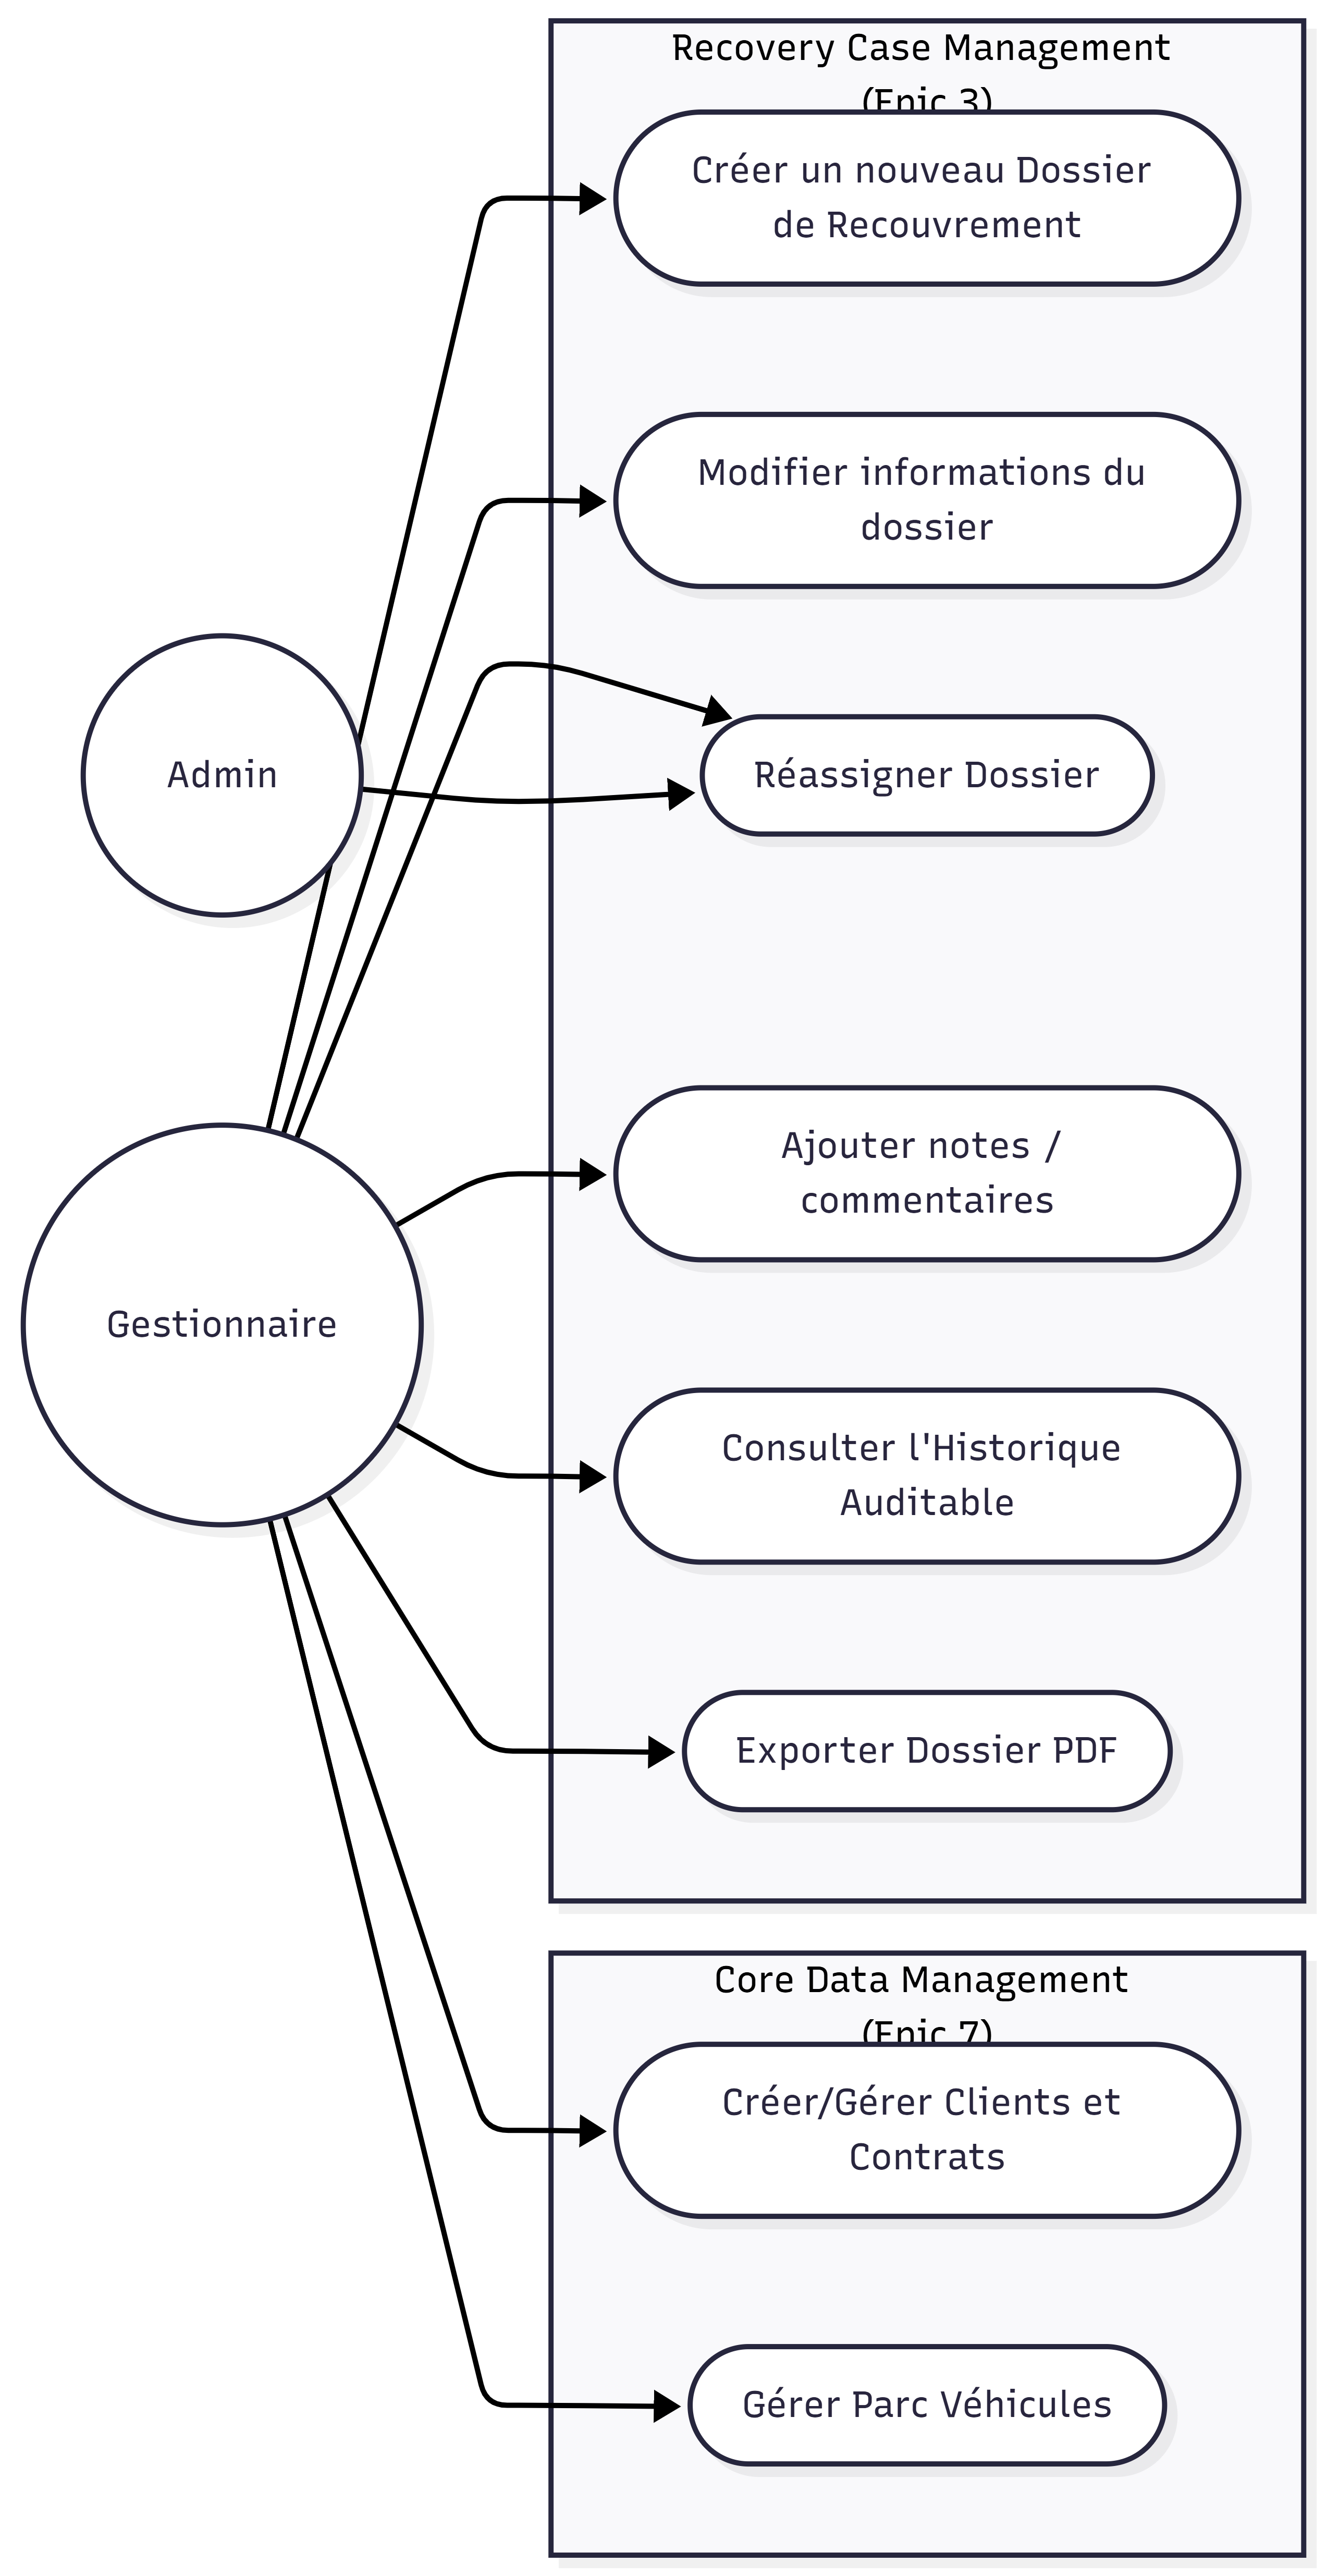
\includegraphics[width=\textwidth,height=0.62\textheight,keepaspectratio]{images/uc2.png}
\caption{Diagramme de cas d'utilisation -- Référentiels Métiers et Dossiers}
\label{fig:uc2_core_cases}
\end{figure}

\begin{itemize}
    \item \textbf{Gestion des Référentiels Métiers (Core Data) :}
    \begin{itemize}
        \item Le \textbf{Gestionnaire de Recouvrement} administre les fiches clients débiteurs (coordonnées, solvabilité), les contrats de crédit-bail associés (valeur résiduelle contractuelle $\vr$, montants impayés) ainsi que le parc de véhicules (numéro VIN, immatriculation, état).
    \end{itemize}
    \item \textbf{Gestion des Dossiers de Recouvrement (Recovery Case Management) :}
    \begin{itemize}
        \item \textit{Création et initialisation :} Ouverture d'un nouveau dossier suite au basculement d'un contrat en défaut de paiement.
        \item \textit{Mise à jour des informations :} Édition des métadonnées du dossier et consignation des événements d'instruction.
        \item \textit{Réassignation de dossier :} Possibilité pour l'\textbf{Administrateur} ou le Gestionnaire de réaffecter la charge d'un dossier à un collègue.
        \item \textit{Annotations et notes de suivi :} Ajout d'observations textuelles et de pièces horodatées.
        \item \textit{Consultation de l'historique et export PDF :} Visualisation de l'historique complet auditable et génération d'un rapport de synthèse imprimable.
    \end{itemize}
\end{itemize}

\clearpage
\subsubsection{Cas d'Utilisation 3 : Workflow Légal, Documents et Pipeline IA}

Le troisième module (figure~\ref{fig:uc3_workflow_ai}) illustre l'interaction entre le gestionnaire opérationnel et les processus automatisés du système et du service IA :

\begin{figure}[H]
\centering

\includegraphics[width=\textwidth,height=0.62\textheight,keepaspectratio]{images/uc3.png}
\caption{Diagramme de cas d'utilisation -- Workflow Légal, Documents et Pipeline IA}
\label{fig:uc3_workflow_ai}
\end{figure}

\begin{itemize}
    \item \textbf{Workflow Légal et Coffre-fort Documentaire :}
    \begin{itemize}
        \item \textit{Téléversement et consultation documentaire :} Le Gestionnaire dépose et archive les pièces probantes (mises en demeure, procès-verbaux d'huissier, rapports d'expertise).
        \item \textit{Progression des phases juridiques :} Le Gestionnaire initie le passage d'une phase à la suivante (\textbf{Pré-contentieux} $\rightarrow$ \textbf{Mise en demeure} $\rightarrow$ \textbf{Saisie} $\rightarrow$ \textbf{Vente} $\rightarrow$ \textbf{Clôture}).
        \item \textit{Contrôle automatisé des prérequis :} Le \textbf{Système} bloque dynamiquement la transition si les documents obligatoires ou les délais minimaux ne sont pas respectés.
        \item \textit{Surveillance des délais légaux :} Le Système émet des alertes proactives à l'approche de la date d'expiration légale d'une phase.
    \end{itemize}
    \item \textbf{Pipeline d'Évaluation Documentaire par Intelligence Artificielle :}
    \begin{itemize}
        \item \textit{Déclenchement du pipeline :} Déclenché manuellement par le Gestionnaire ou automatiquement par le Système lors du téléversement d'un rapport PDF.
        \item \textit{Extraction sémantique NLP/OCR :} Le microservice IA extrait la valeur vénale estimée ($\ve$), le kilométrage et l'état général de l'actif.
        \item \textit{Confrontation financière :} Le Système calcule automatiquement la déviation absolue ($\Delta = \ve - \vr$) et le ratio de couverture ($R$).
        \item \textit{Génération d'indicateur de fiabilité :} Attribution d'un statut décisionnel explicite (\textit{Fiable}, \textit{Écart modéré}, \textit{Écart critique}) guidant le choix d'arbitrage de vente.
    \end{itemize}
\end{itemize}

\clearpage
\subsubsection{Cas d'Utilisation 4 : Command Center, Sécurité et Traçabilité}

Le quatrième module (figure~\ref{fig:uc4_dashboard_security}) regroupe les fonctionnalités du poste de pilotage quotidien ainsi que les mécanismes transversaux de sécurité et d'audit :

\begin{figure}[H]
\centering
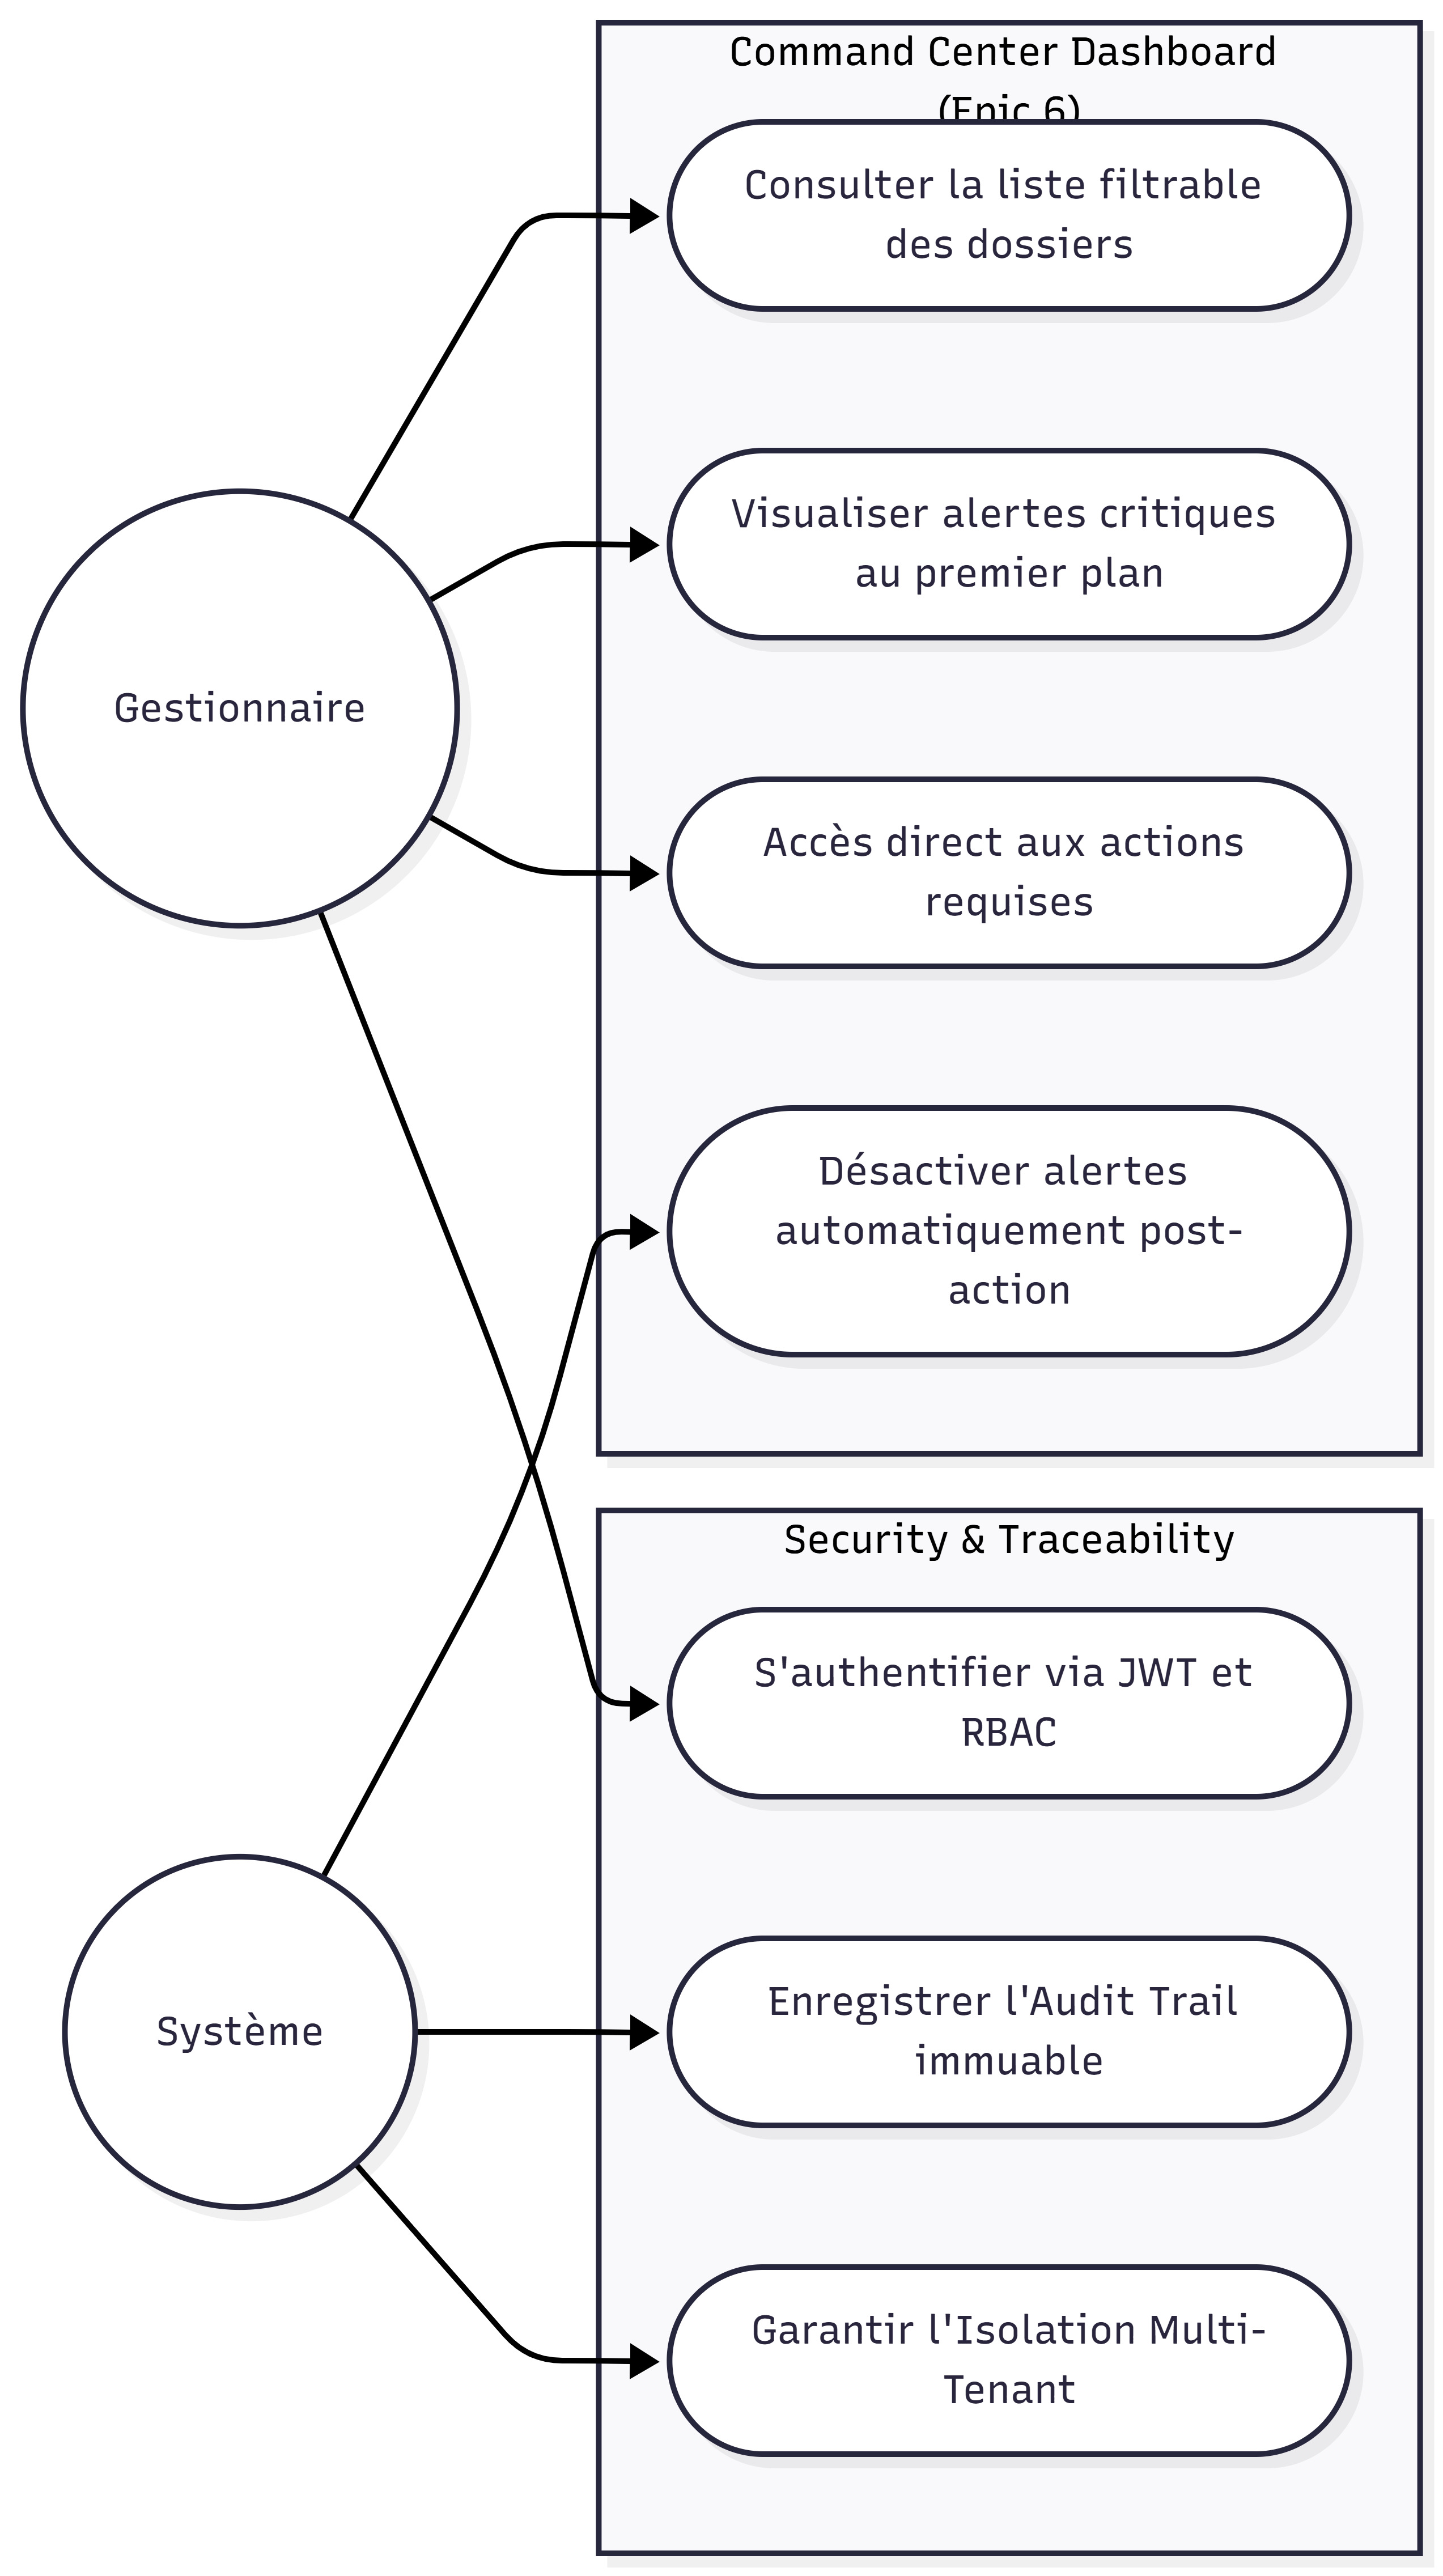
\includegraphics[width=\textwidth,height=0.62\textheight,keepaspectratio]{images/uc4.png}
\caption{Diagramme de cas d'utilisation -- Command Center, Sécurité et Traçabilité}
\label{fig:uc4_dashboard_security}
\end{figure}

\begin{itemize}
    \item \textbf{Tableau de Bord Opérationnel (Command Center Dashboard) :}
    \begin{itemize}
        \item \textit{Registre global filtrable :} Vue unifiée permettant au Gestionnaire de filtrer et trier les dossiers selon la phase, le niveau de criticité ou l'agent assigné.
        \item \textit{Visualisation des alertes critiques :} Mise en évidence des alertes d'expiration de délais légaux, d'anomalies financières IA ou de dormance.
        \item \textit{Accès direct aux actions prioritaires :} Liens d'action rapide permettant d'intervenir immédiatement sur le dossier concerné.
        \item \textit{Désactivation automatique post-action :} Le Système acquitte et clôture les alertes dès l'exécution de l'action corrective requise.
    \end{itemize}
    \item \textbf{Sécurité, Isolation et Traçabilité Système :}
    \begin{itemize}
        \item \textit{Authentification sécurisée et RBAC :} Gestion des sessions par cookies chiffrés et contrôle d'accès strict selon les rôles.
        \item \textit{Piste d'audit immuable (Audit Trail) :} Enregistrement systématique de toutes les créations, modifications et consultations dans un journal infalsifiable.
        \item \textit{Garantie de l'isolation multi-tenant :} Ségrégation stricte des données au niveau de la couche d'accès aux bases de données.
    \end{itemize}
\end{itemize}

\subsection{Diagramme de Classes du Système}

\begin{figure}[H]
\centering

\includegraphics[width=\textwidth,height=2\textheight,keepaspectratio]{images/class_diagram.png}
\caption{Diagramme de classes du système LeasRecover}
\label{fig:class_diagram}
\end{figure}

Le modèle conceptuel de classes (figure~\ref{fig:class_diagram}) respecte les principes d'isolation multi-tenant et de normalisation logicielle :
\begin{itemize}
    \item \textbf{BaseEntity \& TenantAwareEntity :} Classes de base gérant universellement les identifiants uniques (UUID v7), l'audit de création/modification et la clé étrangère \code{tenant_id} fondamentale pour l'étanchéité des données.
    \item \textbf{Entités Métiers :} Classes concrètes modélisant le domaine (\code{Tenant}, \code{User}, \code{RecoveryCase}, \code{Vehicle}, \code{Contract}, \code{AiValuation}, \code{AuditLog}).
\end{itemize}

\section{Planification du Projet}

\subsection{Backlog du Produit}

Le backlog produit a été décomposé en 7 Épiques (\textit{Epics}) fonctionnelles majeures :
\begin{itemize}
    \item \textbf{Epic 1 \& 2 :} Fondations Tenant, Identité et Configuration des politiques de conformité.
    \item \textbf{Epic 3 \& 4 :} Gestion cœur des dossiers, coffre-fort documentaire et respect du workflow légal.
    \item \textbf{Epic 5 \& 6 :} Pipeline d'évaluation intelligente (IA) et Tableau de bord (\textit{Command Center}).
    \item \textbf{Epic 7 :} Référentiels métiers (Clients, Contrats, Véhicules).
\end{itemize}

\clearpage
\subsection{Planification des Sprints et Livrables}

Le projet a été exécuté sur 8 sprints itératifs de deux à trois semaines, détaillés dans le tableau~\ref{tab:planification_sprints}.

\begin{table}[H]
\centering
\small
\caption{Planification des Sprints et Livrables du Projet LeasRecover}
\label{tab:planification_sprints}
\begin{tabularx}{\textwidth}{@{}L{2cm} L{2.2cm} L{6.2cm} Y@{}}
\toprule
\textbf{Sprint} & \textbf{Épique} & \textbf{Objectifs et User Stories} & \textbf{Livrable} \\
\midrule
\textbf{Sprint 1} & Epic 1 (Part. 1) & Initialisation du projet, schéma de base de données global et infrastructure multi-tenant (Stories 1.1, 1.2). & DB prête avec séparation stricte des tenants. \\
\addlinespace
\textbf{Sprint 2} & Epic 1 (Part. 2) & Gestion des utilisateurs, authentification sécurisée via BFF et gestion des sessions (Stories 1.3, 1.4). & Authentification opérationnelle. \\
\addlinespace
\textbf{Sprint 3} & Epic 2 & Politiques de conformité : image de marque, délais légaux, seuils IA (Stories 2.1 à 2.3). & Interface d'administration et règles configurables. \\
\addlinespace
\textbf{Sprint 4} & Epic 7 & Gestion des données de base : Clients, Contrats, Véhicules, documents (Stories 7.1 à 7.3). & Référentiels métiers fonctionnels. \\
\addlinespace
\textbf{Sprint 5} & Epic 3 & Cœur du système : Création/modification des dossiers, Audit Trail (Stories 3.1 à 3.4). & Gestion de l'historique et des dossiers. \\
\addlinespace
\textbf{Sprint 6} & Epic 4 & Workflow légal (5 phases), bloqueurs, alertes et coffre-fort documentaire (Stories 4.1 à 4.4). & Moteur de workflow et alertes de délais. \\
\addlinespace
\textbf{Sprint 7} & Epic 5 & Pipeline IA : Déclencheur API, extraction NLP, comparaison valeur/marché (Stories 5.1 à 5.5). & Module IA d'analyse intégré. \\
\addlinespace
\textbf{Sprint 8} & Epic 6 & Command Center : Registre dossiers, alertes critiques, actions rapides (Stories 6.1 à 6.4). & Tableau de pilotage finalisé. \\
\bottomrule
\end{tabularx}
\end{table}

\clearpage
\section{Architecture de la Solution}

\subsection{Architecture Logique du Système}

L'architecture logique de \projectShortTitle\ repose sur une approche modulaire découpée en trois couches indépendantes (figure~\ref{fig:logic_architecture}) :

\begin{figure}[H]
\centering
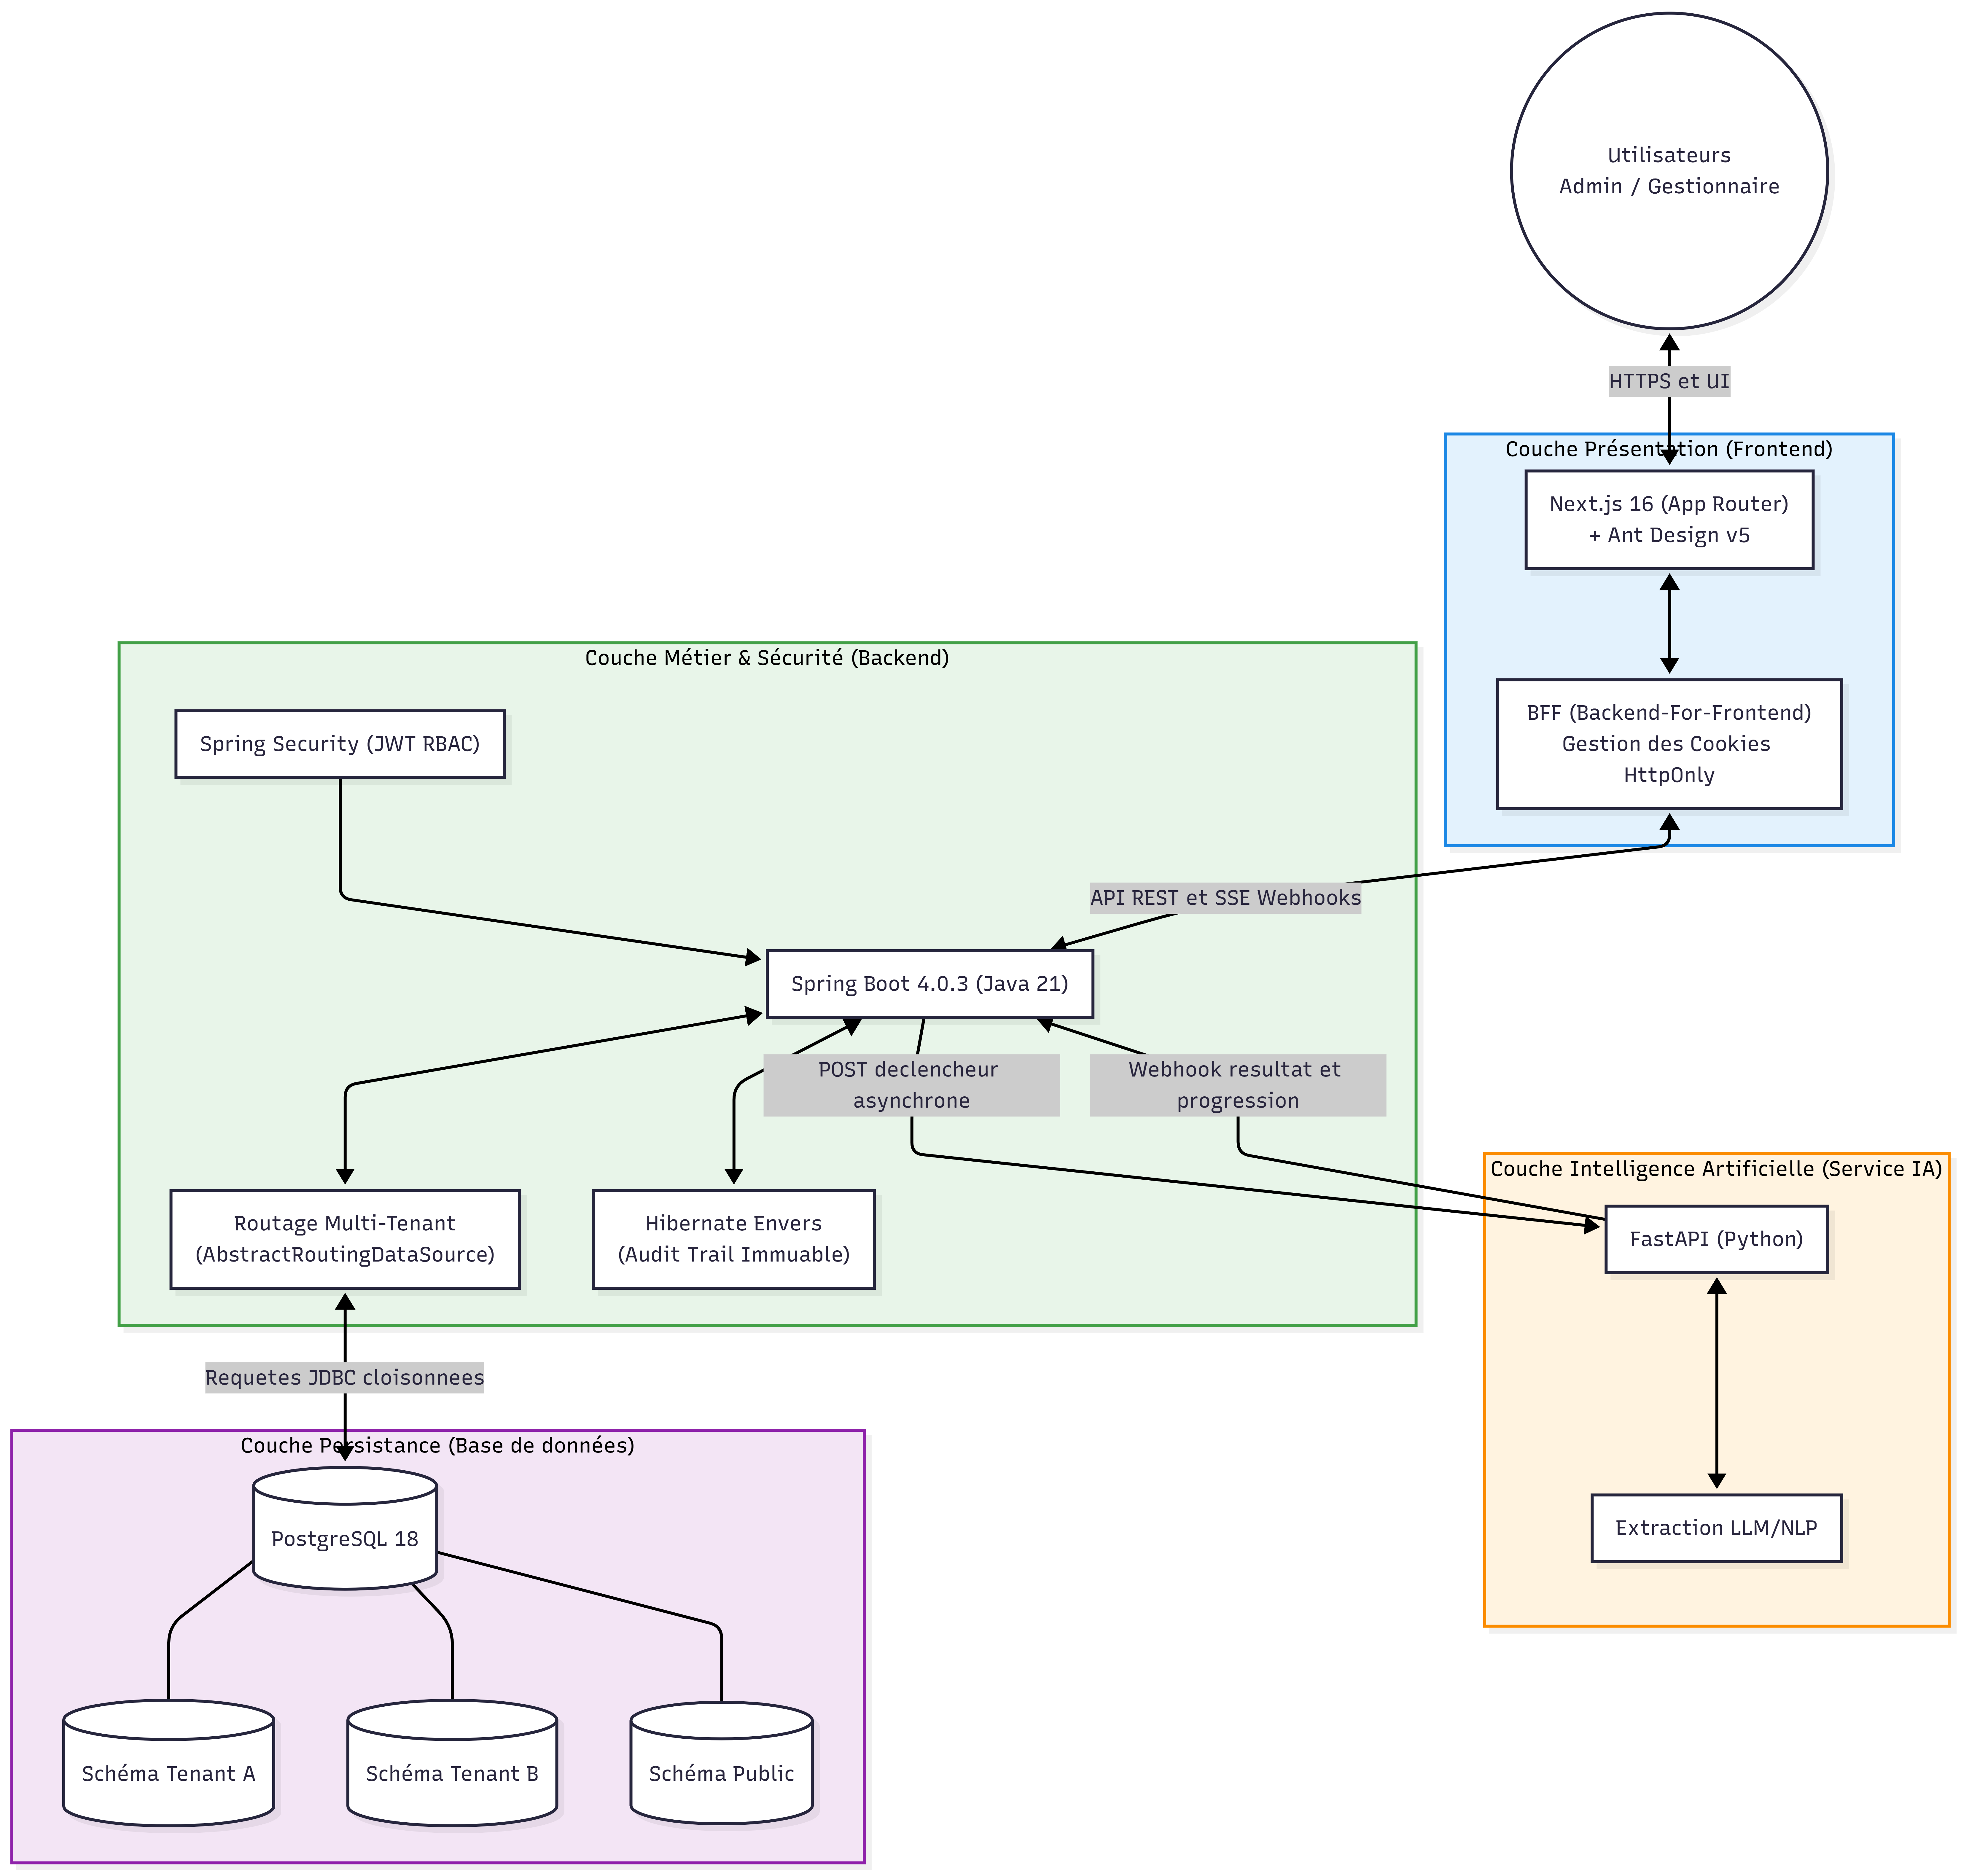
\includegraphics[width=1\textwidth,keepaspectratio]{images/logic-architecture.png}
\caption{Architecture logique du système LeasRecover}
\label{fig:logic_architecture}
\end{figure}

\begin{enumerate}
    \item \textbf{La Couche Présentation (Frontend -- Next.js 16) :} Interface utilisateur réactive développée avec Next.js 16 et la bibliothèque graphique Ant Design. Elle intègre un pattern \textbf{Backend-For-Frontend (BFF)} qui gère de manière invisible et sécurisée les jetons de session (cookies HttpOnly), protégeant ainsi l'application contre les attaques XSS et CSRF.
    \item \textbf{La Couche Métier et Sécurité (Backend -- Spring Boot 4 / Java 21) :} Cœur de l'application. Cette API REST centralise toutes les règles de gestion (workflows, autorisations RBAC, traçabilité). Elle garantit l'isolation multi-tenant en orientant dynamiquement chaque requête vers le schéma de base de données exclusif de la société cliente.
    \item \textbf{La Couche d'Intelligence Artificielle (Service FastAPI / Python) :} Microservice asynchrone haute performance dédié à l'extraction de données complexes (LLM/NLP). Il ingère les rapports d'expertise, extrait les valeurs financières et transmet ses calculs au Backend sans bloquer l'expérience utilisateur.
\end{enumerate}

\subsection{Architecture Physique et Déploiement}

Le déploiement repose sur une infrastructure moderne entièrement conteneurisée. L'ensemble des services (Next.js, Spring Boot, FastAPI) ainsi que la base de données \textbf{PostgreSQL 18} sont encapsulés et orchestrés via \textbf{Docker Compose}. Cette conteneurisation garantit une reproductibilité parfaite et une isolation stricte entre environnements de développement et de production.

\section{Étude de l'environnement}

\subsection{Environnement Matériel}

Le développement a été réalisé sur un poste de travail standard équipé d'un processeur Intel Core i7 et de 16 Go de mémoire vive (RAM), suffisant pour l'orchestration locale des conteneurs Docker et l'exécution des tests.

\subsection{Environnement Logiciel}

\begin{itemize}
    \item \textbf{Next.js 16 \& Ant Design :} Framework React privilégié pour sa robustesse, son routage moderne et ses composants graphiques riches.
    \item \textbf{Spring Boot 4 (Java 21) :} Framework back-end d'entreprise de référence, offrant des fonctionnalités avancées pour la sécurité et la gestion transactionnelle multi-tenant.
    \item \textbf{FastAPI (Python) :} Framework asynchrone haute performance, idéal pour exposer les pipelines d'IA et exécuter les traitements NLP/LLM intensifs.
    \item \textbf{PostgreSQL 18 :} SGBD relationnel robuste choisi pour sa fiabilité transactionnelle ACID et sa gestion efficace des schémas de données isolés.
    \item \textbf{Docker \& Docker Compose :} Outils de virtualisation légère assurant le déploiement cohérent et reproductible des microservices.
\end{itemize}

\clearpage
\section{Conclusion}

Ce chapitre a formalisé de manière exhaustive les exigences fonctionnelles et techniques du système \projectShortTitle. La définition des acteurs, la modélisation UML (diagrammes de cas d'utilisation par module, diagramme de classes), la planification par sprints et l'architecture Next.js / Spring Boot / FastAPI posent un socle particulièrement solide. Le chapitre suivant aborde la conception architecturale détaillée et la modélisation fine des données.

%=============================================================================
% chktex-file 1 chktex-file 8 chktex-file 12 chktex-file 13 chktex-file 24 chktex-file 26
% CHAPITRE 3 : CONCEPTION ARCHITECTURALE ET DÉTAILLÉE
%=============================================================================

\chapter{Conception Architecturale}
\label{chap:conception}

\section{Introduction}

La conception détaillée constitue le pont indispensable entre la spécification des besoins et l'implémentation logicielle. Ce chapitre expose en profondeur les choix d'ingénierie retenus pour la plateforme \textbf{\projectShortTitle}. Nous présentons l'architecture microservices polyglotte, le patron d'isolation multi-tenant à schémas SQL étanches, la modélisation conceptuelle des données (MCD) et relationnelle (MLD), ainsi que la formulation mathématique du moteur d'arbitrage financier.

\section{Architecture Microservices et Flux}

\subsection{Principes de Conception Découplée}

Afin de concilier la robustesse d'un système d'information financier d'entreprise et l'agilité requise pour l'expérimentation d'algorithmes d'intelligence artificielle, nous avons conçu une architecture polyglotte découpée en services spécialisés :

\begin{enumerate}
    \item \textbf{Frontend Next.js 16 (React / TypeScript) :} Fournit l'interface utilisateur enrichie avec Ant Design, orchestrée via le pattern \textbf{Backend-For-Frontend (BFF)}. Le serveur Node.js / Next.js gère la session utilisateur par cookies chiffrés \code{HttpOnly}, \code{SameSite=Strict} et \code{Secure}, éliminant tout stockage vulnérable de jetons JWT dans le \textit{localStorage} du navigateur.
    \item \textbf{Backend Métier Spring Boot 4 (Java 21) :} Constitue le noyau transactionnel de LeasRecover. Il expose une API RESTful sécurisée, applique les règles d'intégrité métier, gère les transitions d'états du workflow de recouvrement et pilote la piste d'audit (\textit{Audit Trail}).
    \item \textbf{Service d'Intelligence Artificielle FastAPI (Python 3.11+) :} Microservice asynchrone spécialisé dans l'ingestion, le prétraitement et l'analyse sémantique des rapports d'expertise de véhicules (LLM / NLP / PyMuPDF).
\end{enumerate}

\subsection{Stratégie d'Isolation Multi-Tenant à Schémas Étanches}

Dans un modèle SaaS B2B destiné à des institutions financières concurrentes, la confidentialité absolue des données est une exigence non négociable. Nous avons retenu l'approche \textbf{Multi-Tenancy par Schémas Séparés (\textit{Schema-per-Tenant})} au sein de PostgreSQL 18 :
\begin{itemize}
    \item Un schéma public \code{shared_platform} centralise les métadonnées globales de la plateforme (annuaire des tenants, plans d'abonnement, configuration système).
    \item Chaque tenant (société de leasing cliente) se voit allouer un schéma SQL dédié et hermétique (ex: \code{tenant_alpha}, \code{tenant_beta}) contenant l'ensemble de ses tables opérationnelles (\code{recovery_cases}, \code{vehicles}, \code{contracts}, \code{audit_logs}).
    \item À chaque requête entrante, un filtre de sécurité Spring Boot extrait l'identifiant du tenant (\code{tenant_id}) depuis le contexte de sécurité et configure dynamiquement le \code{CurrentSchema} de la connexion JDBC via le mécanisme \code{AbstractRoutingDataSource}.
\end{itemize}

Cette approche offre le niveau d'étanchéité le plus élevé, garantissant l'impossibilité technique d'une fuite de données inter-entreprises tout en simplifiant les sauvegardes et la conformité au RGPD.

\section{Modélisation des Données}

La modélisation des données de \textbf{\projectShortTitle} répond aux plus hauts standards de performance, d'intégrité financière et de traçabilité d'audit. Afin de respecter rigoureusement le principe \textbf{DRY (\textit{Don't Repeat Yourself})}, l'architecture logicielle factorise les propriétés communes d'audit, de verrouillage optimiste et d'isolation multi-tenant au travers de classes de base abstraites exploitant le patron \code{@MappedSuperclass} d'Hibernate :
\begin{itemize}
    \item \textbf{BaseEntity :} Classe racine fournissant la clé primaire universelle temporelle (\code{id} en \textbf{UUID v7}, garantissant une indexation B-Tree séquentielle sans fragmentation), les horodatages d'audit (\code{created_at}, \code{updated_at}, \code{created_by}), le contrôle de concurrence optimiste (\code{version}) et le support de la suppression logique (\textit{Soft Delete} via \code{is_deleted} et \code{deleted_at}).
    \item \textbf{TenantAwareEntity :} Hérite de \code{BaseEntity} et adjoint la clé de partitionnement \code{tenant_id} assurant le filtrage étanche des entités rattachées à un établissement financier.
\end{itemize}

Afin d'offrir une clarté de lecture maximale, le Modèle Conceptuel de Données (MCD) est décomposé en trois modules fonctionnels complémentaires.

%-----------------------------------------------------------------------------
\subsection{Module 1 : Administration, Multi-Tenancy et Socle Commun}

Ce module (figure~\ref{fig:mcd_module_admin}) régit la hiérarchie organisationnelle de la plateforme SaaS, l'administration globale et les paramètres d'exploitation spécifiques à chaque société de leasing.

\begin{figure}[H]
\centering
\resizebox{0.95\linewidth}{!}{%
\begin{tikzpicture}[
    node distance=1.3cm and 1.8cm,
    entity/.style={
        rectangle, draw=primaryblue, fill=white, line width=1pt, rounded corners=3pt,
        inner sep=4pt, drop shadow={opacity=0.10, shadow xshift=1.5pt, shadow yshift=-1.5pt}
    },
    baseentity/.style={
        rectangle, draw=darkslate!60, fill=lightgrey!70, line width=0.9pt, dashed, rounded corners=3pt,
        inner sep=4pt
    },
    rel/.style={
        -{Latex[scale=0.9]}, line width=1.1pt, draw=secondaryblue
    },
    inherit/.style={
        -{Triangle[open, scale=0.9]}, line width=1pt, draw=darkslate!70, dashed
    },
    card/.style={
        font=\sffamily\scriptsize\bfseries, fill=white, inner sep=1.5pt, text=darkslate
    },
    relname/.style={
        font=\sffamily\footnotesize\itshape, text=secondaryblue, fill=white, inner sep=1.5pt
    }
]

% Row 2 (Central Business Level): SUPER_ADMIN -> TENANT -> TENANT_CONFIG
\node[entity] (superadmin) {
    \begin{tabular}{l}
        \multicolumn{1}{c}{\textbf{\color{primaryblue} SUPER\_ADMIN}} \\
        \multicolumn{1}{c}{\scriptsize\color{darkslate!70}\guillemotleft extends BaseEntity\guillemotright} \\
        \hline
        \underline{id} : UUID\_v7 \textit{(PK)} \\
        email : String \textit{(Unique)} \\
        password\_hash : String \\
        first\_name, last\_name : String \\
        status : Enum (ACTIVE, SUSPENDED) \\
        last\_login : Timestamp \\
    \end{tabular}
};

\node[entity, right=1.8cm of superadmin] (tenant) {
    \begin{tabular}{l}
        \multicolumn{1}{c}{\textbf{\color{primaryblue} TENANT}} \\
        \multicolumn{1}{c}{\scriptsize\color{darkslate!70}\guillemotleft extends BaseEntity\guillemotright} \\
        \hline
        \underline{id} : UUID\_v7 \textit{(PK)} \\
        name : String \\
        logo\_url : String \\
        data\_retention\_months : Integer \\
        status : Enum (ACTIVE, INACTIVE) \\
    \end{tabular}
};

\node[entity, right=1.8cm of tenant] (tenantcfg) {
    \begin{tabular}{l}
        \multicolumn{1}{c}{\textbf{\color{primaryblue} TENANT\_CONFIG}} \\
        \multicolumn{1}{c}{\scriptsize\color{darkslate!70}\guillemotleft extends TenantAwareEntity\guillemotright} \\
        \hline
        \underline{tenant\_id} : UUID\_v7 \textit{(PK, FK)} \\
        ai\_deviation\_moderate : Decimal \\
        ai\_deviation\_critical : Decimal \\
        dormancy\_threshold\_days : Integer \\
        phase\_legal\_delays : JSONB \\
    \end{tabular}
};

% Row 3 (Bottom): USER under TENANT
\node[entity, below=1.4cm of tenant] (user) {
    \begin{tabular}{l}
        \multicolumn{1}{c}{\textbf{\color{primaryblue} USER}} \\
        \multicolumn{1}{c}{\scriptsize\color{darkslate!70}\guillemotleft extends TenantAwareEntity\guillemotright} \\
        \hline
        \underline{id} : UUID\_v7 \textit{(PK)} \\
        tenant\_id : UUID\_v7 \textit{(FK)} \\
        email : String \textit{(Unique)} \\
        password\_hash : String \\
        first\_name, last\_name : String \\
        role : Enum (ADMIN, GESTIONNAIRE) \\
        status : Enum (ACTIVE, SUSPENDED) \\
        last\_login : Timestamp \\
    \end{tabular}
};

% Row 1 (Top): MappedSuperclasses
\node[baseentity, above=1.3cm of superadmin] (base) {
    \begin{tabular}{l}
        \multicolumn{1}{c}{\textbf{\color{darkslate} \guillemotleft MappedSuperclass\guillemotright\ BaseEntity}} \\
        \hline
        \underline{id} : UUID\_v7 \textit{(PK)} \\
        created\_at, updated\_at : Timestamp \\
        created\_by : String / UUID\_v7 \\
        version : Integer \\
        is\_deleted : Boolean, deleted\_at : Timestamp \\
    \end{tabular}
};

\node[baseentity, above=1.3cm of tenantcfg] (tenantbase) {
    \begin{tabular}{l}
        \multicolumn{1}{c}{\textbf{\color{darkslate} \guillemotleft MappedSuperclass\guillemotright\ TenantAwareEntity}} \\
        \hline
        \textit{(Hérite de BaseEntity)} \\
        tenant\_id : UUID\_v7 \textit{(FK Partition)} \\
    \end{tabular}
};

% Heritage Arrows (Dashed Grey)
\draw[inherit] (tenantbase) -- (base);
\draw[inherit] (superadmin) -- (base);
\draw[inherit] (tenant.north) -- (base.south east);
\draw[inherit] (tenantcfg) -- (tenantbase);
\draw[inherit] (user.east) -| ++(0.9,0) |- (tenantbase.south);

% Business Relations (Solid Blue Arrows)
\draw[rel] (superadmin) -- node[above, relname]{administre} node[pos=0.18, above, card]{1..1} node[pos=0.82, above, card]{0..*} (tenant);
\draw[rel] (tenant) -- node[above, relname]{possède} node[pos=0.18, above, card]{1..1} node[pos=0.82, above, card]{0..1} (tenantcfg);
\draw[rel] (tenant) -- node[right, relname]{emploie} node[pos=0.18, right, card]{1..1} node[pos=0.82, right, card]{0..*} (user);

\end{tikzpicture}%
}
\caption{MCD -- Module 1 : Administration, Multi-Tenancy et Socle d'Héritage}
\label{fig:mcd_module_admin}
\end{figure}

Les caractéristiques clés de ce module comprennent :
\begin{itemize}
    \item \textbf{TENANT :} Représente l'institution financière cliente opérant en espace isolé.
    \item \textbf{TENANT\_CONFIG :} Table de configuration 1:1 paramétrant les seuils de déviation IA (\code{ai_deviation_moderate}, \code{ai_deviation_critical}) et les délais légaux maximaux par phase de recouvrement stockés sous format structuré \textbf{JSONB} indexable.
    \item \textbf{SUPER\_ADMIN \& USER :} Séparation stricte entre les administrateurs de la plateforme SaaS et les collaborateurs métier des bailleurs (\code{ADMIN}, \code{GESTIONNAIRE}).
\end{itemize}

%-----------------------------------------------------------------------------
\subsection{Module 2 : Cœur Métier du Leasing et Gestion des Actifs}

Le deuxième module (figure~\ref{fig:mcd_module_leasing}) modélise les données contractuelles amont issues du Système d'Information du bailleur (clients débiteurs, contrats de financement et véhicules loués).

\begin{figure}[H]
\centering
\resizebox{0.92\linewidth}{!}{%
\begin{tikzpicture}[
    node distance=1.1cm and 1.6cm,
    entity/.style={
        rectangle, draw=primaryblue, fill=white, line width=1pt, rounded corners=3pt,
        inner sep=4pt, drop shadow={opacity=0.10, shadow xshift=1.5pt, shadow yshift=-1.5pt}
    },
    rel/.style={
        -{Latex[scale=0.9]}, line width=1.1pt, draw=secondaryblue
    },
    card/.style={
        font=\sffamily\scriptsize\bfseries, fill=white, inner sep=1.5pt, text=darkslate
    },
    relname/.style={
        font=\sffamily\footnotesize\itshape, text=secondaryblue, fill=white, inner sep=1.5pt
    }
]

% Entities
\node[entity] (client) {
    \begin{tabular}{l}
        \multicolumn{1}{c}{\textbf{\color{primaryblue} CLIENT}} \\
        \hline
        \underline{id} : UUID\_v7 \textit{(PK)} \\
        tenant\_id : UUID\_v7 \textit{(FK)} \\
        full\_name\_or\_company : String \\
        registration\_number : String \\
        contact\_email : String \\
        contact\_phone : String \\
        address : Text \\
    \end{tabular}
};

\node[entity, right=1.6cm of client] (contract) {
    \begin{tabular}{l}
        \multicolumn{1}{c}{\textbf{\color{primaryblue} CONTRACT}} \\
        \hline
        \underline{id} : UUID\_v7 \textit{(PK)} \\
        tenant\_id : UUID\_v7 \textit{(FK)} \\
        client\_id : UUID\_v7 \textit{(FK)} \\
        reference\_number : String \textit{(Unique)} \\
        start\_date, end\_date : Timestamp \\
        status : Enum (ACTIVE, DEFAULTED, ...) \\
    \end{tabular}
};

\node[entity, below=1.2cm of contract] (vehicle) {
    \begin{tabular}{l}
        \multicolumn{1}{c}{\textbf{\color{primaryblue} VEHICLE}} \\
        \hline
        \underline{id} : UUID\_v7 \textit{(PK)} \\
        tenant\_id : UUID\_v7 \textit{(FK)} \\
        contract\_id : UUID\_v7 \textit{(FK)} \\
        vin : String \textit{(Unique, 17 cars)} \\
        license\_plate : String \\
        brand, model : String \\
        year : Integer \\
    \end{tabular}
};

% Relations
\draw[rel] (client) -- node[above, relname]{signe} node[pos=0.1, above, card]{1..1} node[pos=0.9, above, card]{0..*} (contract);
\draw[rel] (contract) -- node[right, relname]{concerne} node[pos=0.1, right, card]{1..1} node[pos=0.9, right, card]{0..1} (vehicle);

\end{tikzpicture}%
}
\caption{MCD -- Module 2 : Gestion Métier du Leasing et des Véhicules}
\label{fig:mcd_module_leasing}
\end{figure}

Chaque contrat de leasing relie de manière univoque un débiteur (\code{CLIENT}) à l'actif financé (\code{VEHICLE}) identifié par son numéro de châssis unique (\code{vin}).

%-----------------------------------------------------------------------------
\subsection{Module 3 : Recouvrement Contentieux, Documents et Évaluation IA}

Le troisième module (figure~\ref{fig:mcd_module_recovery_ai}) constitue le noyau opérationnel de LeasRecover. Il orchestre les dossiers de recouvrement en contentieux, les documents d'expertise, les annotations des gestionnaires et l'inférence du moteur d'estimation IA.

\begin{figure}[H]
\centering
\resizebox{0.95\linewidth}{!}{%
\begin{tikzpicture}[
    node distance=1.2cm and 1.6cm,
    entity/.style={
        rectangle, draw=primaryblue, fill=white, line width=1pt, rounded corners=3pt,
        inner sep=4pt, drop shadow={opacity=0.10, shadow xshift=1.5pt, shadow yshift=-1.5pt}
    },
    rel/.style={
        -{Latex[scale=0.9]}, line width=1.1pt, draw=secondaryblue
    },
    card/.style={
        font=\sffamily\scriptsize\bfseries, fill=white, inner sep=1.5pt, text=darkslate
    },
    relname/.style={
        font=\sffamily\footnotesize\itshape, text=secondaryblue, fill=white, inner sep=1.5pt
    }
]

% Central Case Entity (Top Left)
\node[entity] (case) {
    \begin{tabular}{l}
        \multicolumn{1}{c}{\textbf{\color{primaryblue} RECOVERY\_CASE}} \\
        \hline
        \underline{id} : UUID\_v7 \textit{(PK)} \\
        tenant\_id : UUID\_v7 \textit{(FK)} \\
        assignee\_id : UUID\_v7 \textit{(FK User)} \\
        contract\_id : UUID\_v7 \textit{(FK Contract)} \\
        initial\_residual\_value\_cents : BigInt \\
        currency\_code : String(3) \\
        current\_phase : Enum (PRE\_CONTENTIEUX, ...) \\
        phase\_started\_at, last\_action\_at : Timestamp \\
        status : Enum (ACTIVE, CLOSED, CANCELLED) \\
    \end{tabular}
};

% Documents (Top Right)
\node[entity, right=1.6cm of case] (doc) {
    \begin{tabular}{l}
        \multicolumn{1}{c}{\textbf{\color{primaryblue} DOCUMENT}} \\
        \hline
        \underline{id} : UUID\_v7 \textit{(PK)} \\
        tenant\_id : UUID\_v7 \textit{(FK)} \\
        uploader\_id : UUID\_v7 \textit{(FK User)} \\
        case\_id : UUID\_v7 \textit{(FK nullable)} \\
        client\_id, contract\_id, vehicle\_id : UUID\_v7 \\
        file\_name, file\_url : String \\
        phase\_uploaded\_in : Enum \textit{(nullable)} \\
    \end{tabular}
};

% Note (Bottom Left)
\node[entity, below=1.2cm of case] (note) {
    \begin{tabular}{l}
        \multicolumn{1}{c}{\textbf{\color{primaryblue} NOTE}} \\
        \hline
        \underline{id} : UUID\_v7 \textit{(PK)} \\
        tenant\_id : UUID\_v7 \textit{(FK)} \\
        case\_id : UUID\_v7 \textit{(FK)} \\
        author\_id : UUID\_v7 \textit{(FK User)} \\
        content : Text \\
    \end{tabular}
};

% AI Valuation (Bottom Right)
\node[entity, below=1.2cm of doc] (ai) {
    \begin{tabular}{l}
        \multicolumn{1}{c}{\textbf{\color{primaryblue} AI\_VALUATION}} \\
        \hline
        \underline{id} : UUID\_v7 \textit{(PK)} \\
        tenant\_id : UUID\_v7 \textit{(FK)} \\
        case\_id : UUID\_v7 \textit{(FK)} \\
        document\_id : UUID\_v7 \textit{(FK nullable)} \\
        extracted\_brand, extracted\_model : String \\
        extracted\_year, extracted\_mileage : Integer \\
        extracted\_condition : String \\
        estimated\_market\_value\_cents : BigInt \\
        deviation\_value\_cents : BigInt \\
        deviation\_percentage : Decimal \\
        reliability\_indicator : Enum (RELIABLE, ...) \\
        status : Enum (PENDING, SUCCESS, FAILED) \\
        processed\_at : Timestamp \\
    \end{tabular}
};

% Relations
\draw[rel] (case) -- node[above, relname]{contient} node[pos=0.1, above, card]{1..1} node[pos=0.9, above, card]{0..*} (doc);
\draw[rel] (case) -- node[right, relname]{commenté par} node[pos=0.1, right, card]{1..1} node[pos=0.9, right, card]{0..*} (note);
\draw[rel] (case) -- node[above, sloped, relname]{évalué par} node[pos=0.1, above, card]{1..1} node[pos=0.9, above, card]{0..*} (ai);
\draw[rel] (doc) -- node[right, relname]{analysé dans} node[pos=0.1, right, card]{0..1} node[pos=0.9, right, card]{0..1} (ai);

\end{tikzpicture}%
}
\caption{MCD -- Module 3 : Recouvrement Contentieux, Pièces Jointes et Estimation IA}
\label{fig:mcd_module_recovery_ai}
\end{figure}

Ce module intègre des optimisations financières et techniques déterminantes :
\begin{itemize}
    \item \textbf{Typage Monétaire Strict (\code{BigInt}) :} Les montants financiers (\code{initial_residual_value_cents}, \code{estimated_market_value_cents}, \code{deviation_value_cents}) sont enregistrés en centimes afin d'exclure toute erreur d'arrondi en virgule flottante.
    \item \textbf{Liaison Polymorphique des Documents :} L'entité \code{DOCUMENT} dispose de clés étrangères optionnelles vers le dossier, le contrat, le client ou le véhicule, permettant le rattachement transverse des pièces justificatives.
    \item \textbf{Piste d'Audit Automatisée via Hibernate Envers :} L'historisation intégrale des modifications de statuts et de phases n'encombre pas le MCD opérationnel : toute entité annotée \code{@Audited} génère automatiquement sa table miroir d'audit (\code{RECOVERY_CASE_AUD}) avec traçabilité de l'auteur et des valeurs modifiées.
\end{itemize}

%-----------------------------------------------------------------------------
\subsection{Modèle Logique des Données (MLD)}

La transcription relationnelle normalisée en Troisième Forme Normale (3NF) avec application de la stratégie \code{@MappedSuperclass} génère les schémas relationnels suivants :

\begin{sloppypar}
\begin{itemize}
\raggedright
    \item \textbf{tenants} (\underline{id}, name, logo\_url, data\_retention\_months, status, is\_deleted, deleted\_at, created\_at, updated\_at, created\_by, version)
    \item \textbf{tenant\_configs} (\underline{tenant\_id}\#, ai\_deviation\_moderate, ai\_deviation\_critical, dormancy\_threshold\_days, phase\_legal\_delays, is\_deleted, deleted\_at, created\_at, updated\_at, created\_by, version)
    \item \textbf{super\_admins} (\underline{id}, email, password\_hash, first\_name, last\_name, status, last\_login, is\_deleted, deleted\_at, created\_at, updated\_at, created\_by, version)
    \item \textbf{users} (\underline{id}, email, password\_hash, first\_name, last\_name, role, status, last\_login, is\_deleted, deleted\_at, created\_at, updated\_at, created\_by, version, \textit{tenant\_id}\#)
    \item \textbf{clients} (\underline{id}, full\_name\_or\_company, registration\_number, contact\_email, contact\_phone, address, is\_deleted, deleted\_at, created\_at, updated\_at, created\_by, version, \textit{tenant\_id}\#)
    \item \textbf{contracts} (\underline{id}, reference\_number, start\_date, end\_date, status, is\_deleted, deleted\_at, created\_at, updated\_at, created\_by, version, \textit{client\_id}\#, \textit{tenant\_id}\#)
    \item \textbf{vehicles} (\underline{id}, vin, license\_plate, brand, model, year, is\_deleted, deleted\_at, created\_at, updated\_at, created\_by, version, \textit{contract\_id}\#, \textit{tenant\_id}\#)
    \item \textbf{recovery\_cases} (\underline{id}, initial\_residual\_value\_cents, currency\_code, current\_phase, phase\_started\_at, last\_action\_at, status, is\_deleted, deleted\_at, created\_at, updated\_at, created\_by, version, \textit{contract\_id}\#, \textit{assignee\_id}\#, \textit{tenant\_id}\#)
    \item \textbf{documents} (\underline{id}, file\_name, file\_url, phase\_uploaded\_in, is\_deleted, deleted\_at, created\_at, updated\_at, created\_by, version, \textit{uploader\_id}\#, \textit{case\_id}\#, \textit{client\_id}\#, \textit{contract\_id}\#, \textit{vehicle\_id}\#, \textit{tenant\_id}\#)
    \item \textbf{notes} (\underline{id}, content, is\_deleted, deleted\_at, created\_at, updated\_at, created\_by, version, \textit{case\_id}\#, \textit{author\_id}\#, \textit{tenant\_id}\#)
    \item \textbf{ai\_valuations} (\underline{id}, extracted\_brand, extracted\_model, extracted\_year, extracted\_mileage, extracted\_condition, estimated\_market\_value\_cents, currency\_code, deviation\_value\_cents, deviation\_percentage, reliability\_indicator, status, processed\_at, is\_deleted, deleted\_at, created\_at, updated\_at, created\_by, version, \textit{case\_id}\#, \textit{document\_id}\#, \textit{tenant\_id}\#)
\end{itemize}
\end{sloppypar}

\section{Conception du Moteur d'Arbitrage Financier}

L'arbitrage financier constitue le cœur de la valeur ajoutée décisionnelle de \projectShortTitle. Dès la réception des valeurs extraites par le module d'intelligence artificielle, le système exécute le calcul de la déviation absolue ($\Delta$) et du ratio de couverture ($R$) :

\begin{equation}
    \Delta = \ve - \vr
\end{equation}
\begin{equation}
    R = \left( \frac{\ve}{\vr} \right) \times 100\%
\end{equation}

Trois catégories d'arbitrage sont alors automatiquement déterminées par le moteur de règles :
\begin{enumerate}
    \item \textbf{Zone Verte -- Arbitrage Favorable ($R \ge 100\%$) :} La valeur vénale marchande de l'actif couvre ou dépasse la valeur résiduelle comptable. La vente peut être immédiatement autorisée sans perte financière pour le bailleur.
    \item \textbf{Zone Orange -- Écart Modéré ($75\% \le R < 100\%$) :} Une dépréciation modérée est constatée. Une provision pour dépréciation équivalente au montant $|\Delta|$ est automatiquement suggérée au service financier.
    \item \textbf{Zone Rouge -- Écart Critique ($R < 75\%$) :} Dégradation sévère du véhicule ou kilométrage excessif. Le système déclenche une alerte prioritaire et exige une double approbation hiérarchique avant fixation du prix de réserve de cession.
\end{enumerate}

\section{Conclusion}

Ce chapitre a approfondi l'architecture logicielle de la plateforme \projectShortTitle. L'isolation par schémas PostgreSQL, le découplage des couches Next.js / Spring Boot / FastAPI, la normalisation du modèle de données (MCD/MLD) et la modélisation mathématique du moteur d'arbitrage financier posent les bases d'une implémentation robuste. Le chapitre suivant présente la réalisation concrète, le code du pipeline IA, les interfaces utilisateurs et la validation expérimentale du système.


%=============================================================================
% chktex-file 1 chktex-file 8 chktex-file 12 chktex-file 13 chktex-file 24 chktex-file 26
% CHAPITRE 4 : RÉALISATION ET IMPLÉMENTATION
%=============================================================================

\chapter{Réalisation, Pipeline IA et Validation}
\label{chap:realisation}

\section{Introduction}

Ce quatrième chapitre détaille la concrétisation logicielle de la plateforme \textbf{\projectShortTitle}. Nous présentons d'abord l'environnement de développement et de déploiement, puis nous détaillons le fonctionnement du pipeline d'intelligence artificielle dédié à l'analyse des rapports d'expertise. Nous exposons ensuite les principales interfaces utilisateurs conçues, avant de conclure par la méthodologie de test et les résultats de la validation expérimentale.

\section{Environnement Technologique et Outils de Développement}

La réalisation du projet s'appuie sur une pile logicielle moderne et complémentaire, résumée dans le tableau~\ref{tab:tech_stack}.

\begin{table}[H]
\centering
\small
\caption{Synthèse de la pile technologique de la plateforme LeasRecover}
\label{tab:tech_stack}
\begin{tabularx}{\textwidth}{@{}L{3.5cm} L{3.5cm} Y@{}}
\toprule
\textbf{Couche / Domaine} & \textbf{Technologie} & \textbf{Rôle et Justification} \\
\midrule
\textbf{Interface Utilisateur} & Next.js 16 (React, TypeScript) & Rendu hybride rapide, typage statique strict et intégration de la bibliothèque Ant Design. \\
\addlinespace
\textbf{Couche BFF (Sécurité)} & Node.js / Next.js Server & Gestion sécurisée des sessions par cookies chiffrés \code{HttpOnly} sans exposition de tokens. \\
\addlinespace
\textbf{Noyau Métier Backend} & Spring Boot 4 (Java 21) & Gestion transactionnelle robuste, moteur de workflow et routage dynamique multi-tenant. \\
\addlinespace
\textbf{Service IA \& NLP} & FastAPI (Python 3.11+) & Microservice asynchrone pour le traitement documentaire, PyMuPDF et modèles LLM. \\
\addlinespace
\textbf{Persistance} & PostgreSQL 18 & Base de données relationnelle avec schémas séparés par tenant et intégrité ACID. \\
\addlinespace
\textbf{Conteneurisation} & Docker \& Docker Compose & Orchestration unifiée garantissant l'isolation des microservices et la portabilité. \\
\bottomrule
\end{tabularx}
\end{table}

\section{Implémentation du Pipeline IA}

\subsection{Architecture du Pipeline Asynchrone}

L'ingestion et l'analyse d'un rapport d'expertise PDF non structuré s'exécutent selon une chaîne de traitement asynchrone représentée dans la figure~\ref{fig:pipeline_ia}.

\begin{figure}[H]
\centering
\begin{tikzpicture}[
    scale=0.78, every node/.style={transform shape},
    node distance=1.2cm and 1.4cm,
    stepbox/.style={
        rectangle, draw=primaryblue, fill=lightgrey, line width=1.1pt, rounded corners=5pt,
        minimum width=2.8cm, minimum height=1.3cm, align=center, font=\sffamily\small, drop shadow
    },
    flowarrow/.style={
        -{Stealth[scale=1.1]}, line width=1.3pt, color=secondaryblue
    }
]

% Nodes
\node[stepbox, fill=accentorange!15] (docIn) {\textbf{Ingestion}\\[2pt]Rapport PDF\\(Scan / Vecteur)};
\node[stepbox, fill=primaryblue!15, right=of docIn] (preproc) {\textbf{Prétraitement}\\[2pt]Extraction PyMuPDF\\\& Binarisation};
\node[stepbox, fill=secondaryblue!15, right=of preproc] (extract) {\textbf{Extraction Sémantique}\\[2pt]NLP / LLM Parsing\\\& Regex Montants};
\node[stepbox, fill=accentgreen!15, right=of extract] (decision) {\textbf{Rapprochement}\\[2pt]Calcul $\Delta = \ve - \vr$\\Indicateur Tripartite};

% Connections
\draw[flowarrow] (docIn) -- (preproc);
\draw[flowarrow] (preproc) -- (extract);
\draw[flowarrow] (extract) -- (decision);

\end{tikzpicture}
\caption{Pipeline d'ingestion et d'extraction IA des rapports d'expertise}
\label{fig:pipeline_ia}
\end{figure}

\subsection{Algorithme d'Extraction et de Confrontation Financière}

L'algorithme~\ref{alg:extraction_ia} résume le processus d'analyse documentaire, d'extraction des métriques clés (valeur vénale estimée $\ve$, kilométrage, frais de remise en état) et de calcul du score de fiabilité.

\begin{algorithm}[H]
\caption{Algorithme d'extraction et de validation des données d'expertise}
\label{alg:extraction_ia}
\begin{algorithmic}[1]
\REQUIRE Document PDF $D$, Valeur résiduelle contractuelle $\vr$
\ENSURE Tuple $(\ve, \text{Kilométrage}, \Delta, \text{Fiabilité}, \text{ScoreConfiance})$
\STATE $\text{TexteBrut} \leftarrow \text{PyMuPDF\_Extract}(D)$
\IF{$\text{Longueur}(\text{TexteBrut}) < 50$}
    \STATE $\text{TexteBrut} \leftarrow \text{OCR\_Fallback}(D)$
\ENDIF
\STATE $\ve \leftarrow \text{ExtraireEntitéFinancière}(\text{TexteBrut}, \text{cible}=\text{« valeur »})$
\STATE $\text{Km} \leftarrow \text{ExtraireEntier}(\text{TexteBrut}, \text{cible}=\text{« kilométrage »})$
\STATE $\text{Frais} \leftarrow \text{ExtraireMontant}(\text{TexteBrut}, \text{cible}=\text{« frais »})$
\STATE $\text{ScoreConfiance} \leftarrow \text{CalculerScore}(\ve, \text{Km}, \text{TexteBrut})$
\STATE $\Delta \leftarrow \ve - \vr$
\STATE $\text{Ratio} \leftarrow (\ve / \vr) \times 100\%$
\IF{$\text{Ratio} \ge 100\%$}
    \STATE $\text{Fiabilité} \leftarrow \text{« Favorable (Vert) »}$
\ELSIF{$\text{Ratio} \ge 75\%$}
    \STATE $\text{Fiabilité} \leftarrow \text{« Écart Modéré (Orange) »}$
\ELSE
    \STATE $\text{Fiabilité} \leftarrow \text{« Écart Critique (Rouge) »}$
\ENDIF
\RETURN $(\ve, \text{Km}, \Delta, \text{Fiabilité}, \text{ScoreConfiance})$
\end{algorithmic}
\end{algorithm}

\section{Présentation des Interfaces Utilisateurs}
\label{sec:interfaces}

L'ergonomie et le design de la plateforme \textbf{\projectShortTitle} ont été spécifiquement conçus pour répondre aux exigences des gestionnaires de recouvrement et des analystes financiers en contexte institutionnel. L'interface privilégie une hiérarchisation stricte de l'information (\textit{Urgency First}), une réduction maximale de la charge cognitive et une transparence décisionnelle totale. Cette section détaille les écrans majeurs développés pour la solution.

%------------------------------------------------------------------------------
\subsection{Écran d'Authentification et Contrôle d'Accès Sécurisé}
\label{subsec:screen_login}

L'écran de connexion (Figure~\ref{fig:screen_login}) constitue le point d'entrée unique de la plateforme pour deux populations distinctes grâce à un sélecteur segmenté (\textit{Société (Tenant)} / \textit{Super Administration}) :
\begin{itemize}
    \item \textbf{Espace Société :} Le gestionnaire saisit l'identifiant unique de son organisation (\code{Tenant UUID}), son adresse électronique et son mot de passe.
    \item \textbf{Super Administration :} Dédié aux administrateurs de la plateforme pour le provisioning des sociétés de leasing partenaires, sans accès aux données confidentielles des dossiers.
\end{itemize}

Sur le plan technique et sécuritaire, cette interface s'appuie sur le modèle \acro{BFF}{Backend-for-Frontend} de Next.js. Lors de la validation des identifiants, un cookie chiffré \code{HttpOnly} et \code{SameSite=Strict} est injecté dans le navigateur de l'utilisateur. Aucun jeton sensible (JWT) n'est stocké dans le \code{localStorage}, immunisant ainsi l'application contre les attaques de type \acro{XSS}{Cross-Site Scripting}.

\begin{figure}[H]
\centering
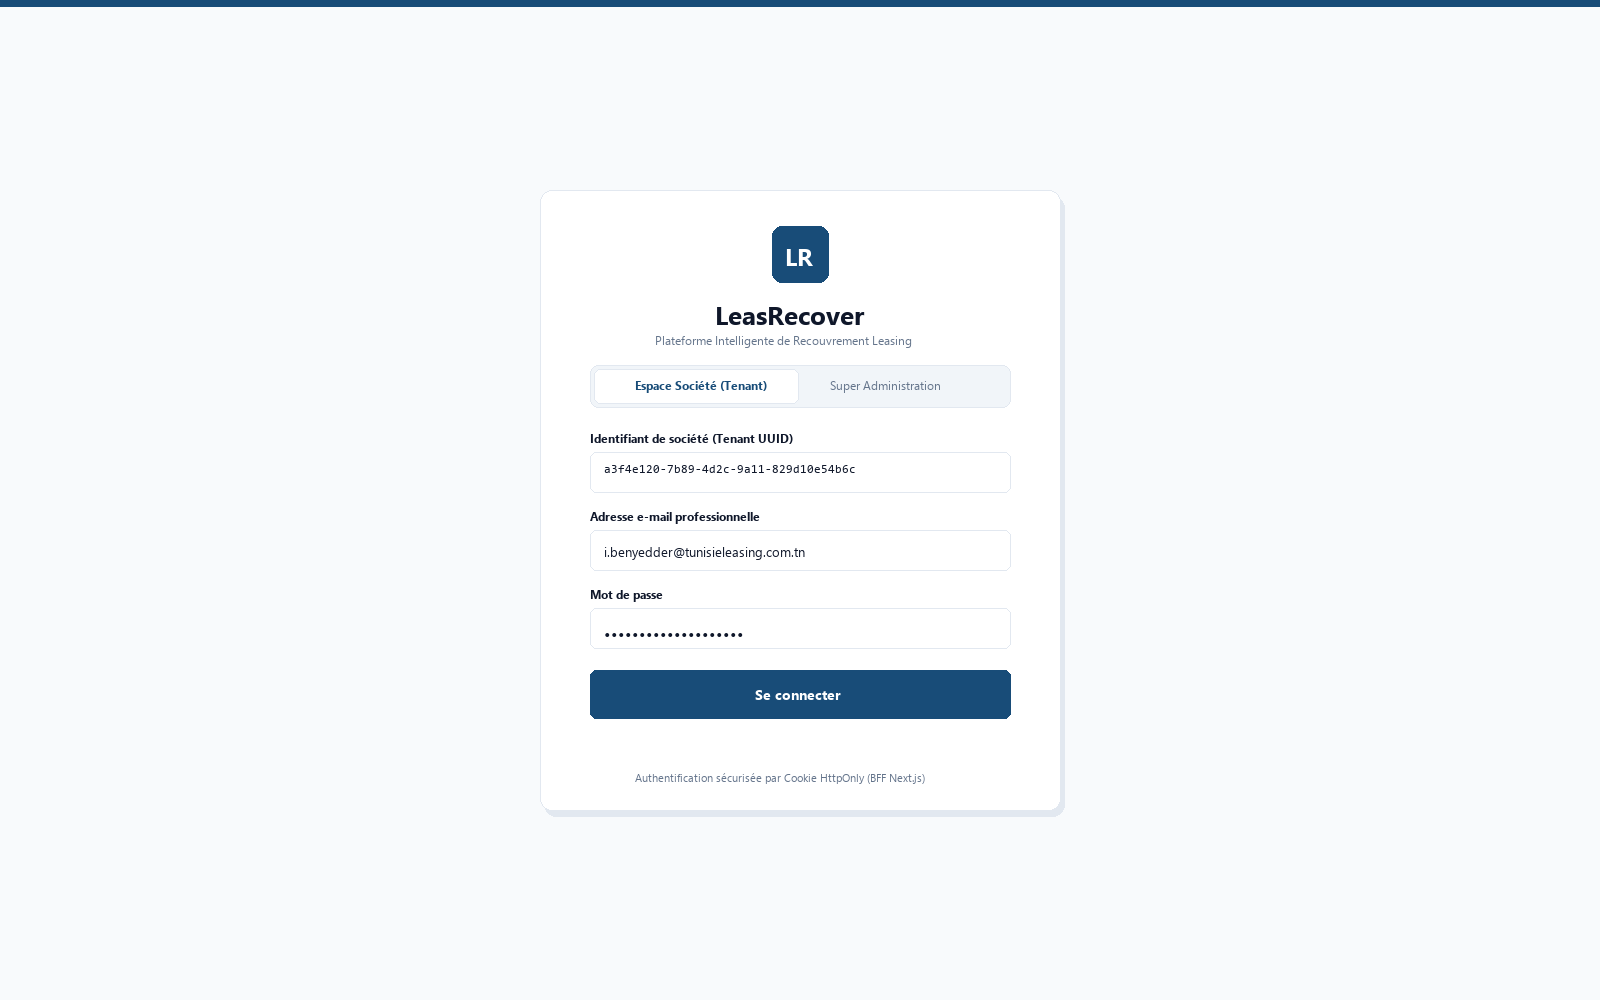
\includegraphics[width=0.92\textwidth,keepaspectratio]{images/screen_login.png}
\caption{Écran d'authentification sécurisée multi-tenant avec isolation BFF}
\label{fig:screen_login}
\end{figure}

%------------------------------------------------------------------------------
\subsection{Tableau de Bord de Pilotage et Registre des Dossiers (Command Center)}
\label{subsec:screen_dashboard}

Le tableau de bord (Figure~\ref{fig:screen_dashboard}) représente le centre névralgique du gestionnaire de recouvrement. Il centralise la totalité du portefeuille de contentieux et hiérarchise immédiatement les urgences opérationnelles :
\begin{itemize}
    \item \textbf{Indicateurs de Synthèse (KPIs) :} Visualisation en temps réel du nombre total de dossiers actifs (62 dossiers), du montant global des valeurs résiduelles en risque (2\,840\,500~TND), des échéances légales imminentes et du taux d'automatisation des arbitrages IA (94.8\,\%).
    \item \textbf{Flux d'Alertes Prioritaires :} Bandeau dynamique situé au sommet de la page, mettant en exergue les dossiers nécessitant une intervention urgente (délais légaux sous 48h, dormance critique de dossiers sans action depuis plus de 21 jours). Chaque alerte offre un bouton d'action contextuel permettant de sauter directement à l'étape requise.
    \item \textbf{Barre de Recherche et Filtrage à Facettes :} Recherche textuelle instantanée (client, référence, immatriculation) et filtres combinables par phase de recouvrement, statut et fiabilité de l'expertise IA.
    \item \textbf{Registre Tabulaire Paginé :} Tableau à haute densité d'information présentant l'état d'avancement, le gestionnaire affecté, la valeur résiduelle et le badge de fiabilité issu du pipeline IA.
\end{itemize}

\begin{figure}[H]
\centering
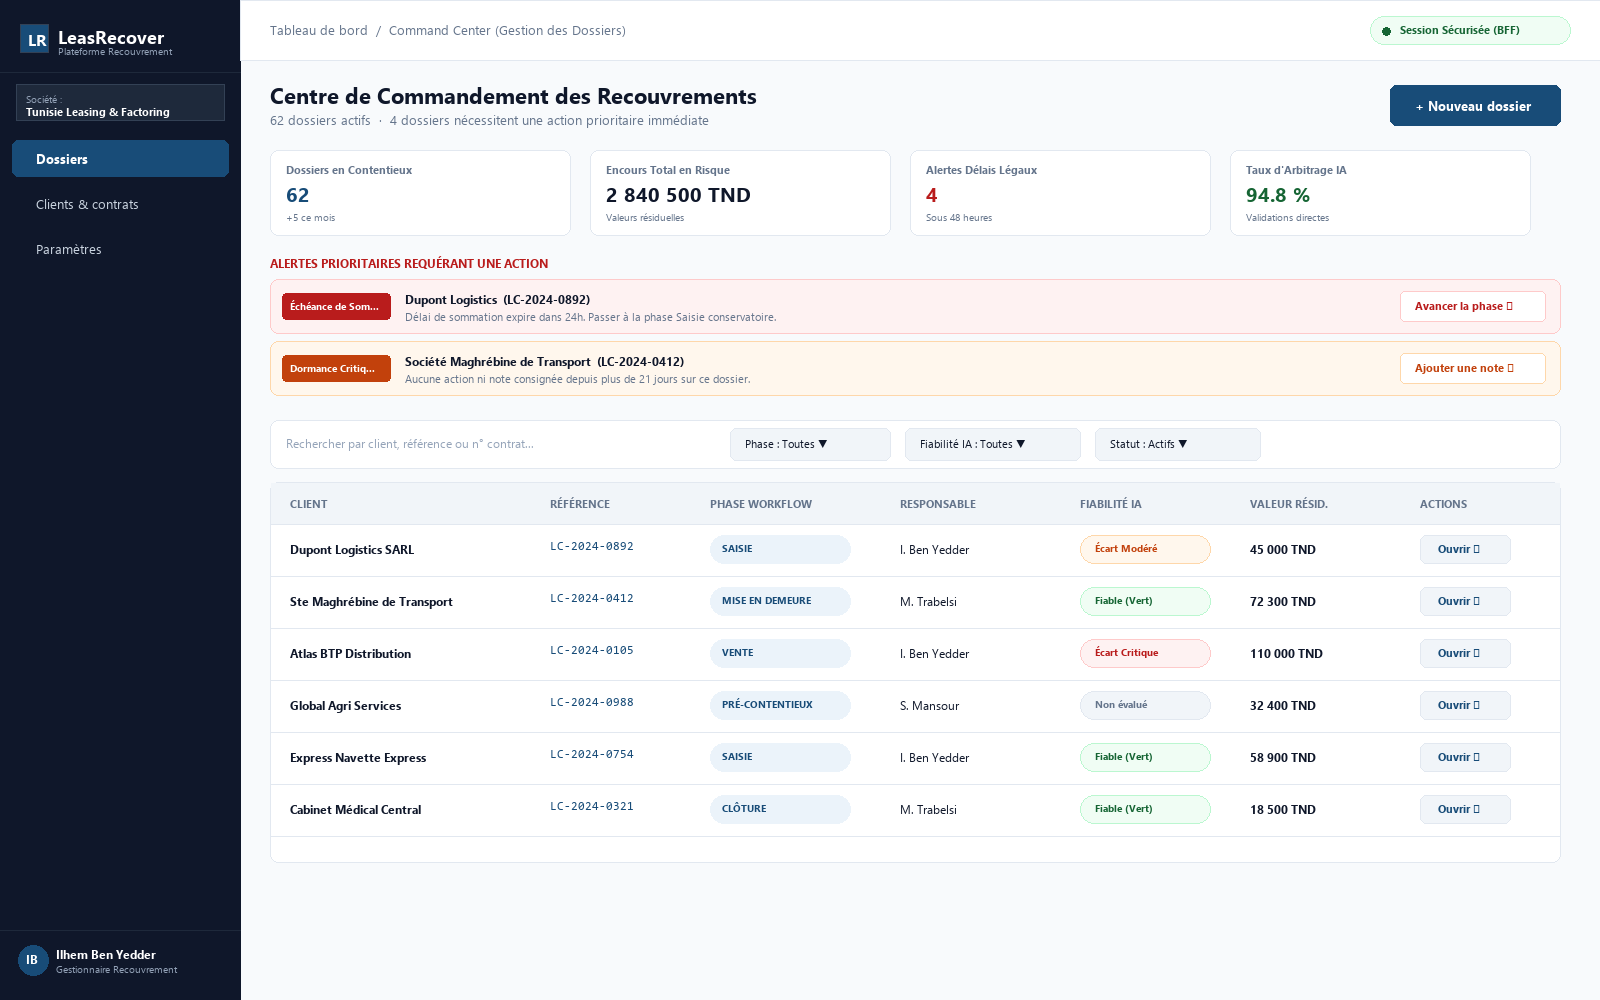
\includegraphics[width=0.95\textwidth,keepaspectratio]{images/screen_dashboard.png}
\caption{Centre de commandement (\textit{Command Center}) et flux d'alertes proactives}
\label{fig:screen_dashboard}
\end{figure}

%------------------------------------------------------------------------------
\subsection{Fiche Dossier Interactive et Moteur de Workflow Métier}
\label{subsec:screen_case_detail}

La vue détaillée d'un dossier de recouvrement (Figure~\ref{fig:screen_case_detail}) orchestre le cycle de vie complet du contentieux autour des cinq phases juridiques obligatoires :
\begin{itemize}
    \item \textbf{Barre de Progression Interactive (\textit{Phase Stepper}) :} Positionne visuellement le dossier au sein des cinq jalons (\textit{1. Pré-contentieux}, \textit{2. Mise en demeure}, \textit{3. Saisie}, \textit{4. Vente}, \textit{5. Clôture}). Les étapes validées sont marquées en vert, la phase courante en bleu primaire, et les étapes futures sous cadenas.
    \item \textbf{Gestion des Prérequis et Verrous Bloquants :} Le moteur de règles évalue dynamiquement les conditions nécessaires pour franchir une étape. En cas d'incomplétude (par exemple, absence du rapport d'expertise ou de l'ordonnance de saisie), une bannière explicite indique précisément la pièce manquante et désactive l'avancement.
    \item \textbf{Volet Latéral Persistant (\textit{Sticky Aside}) :} Synthétise les informations financières fondamentales (valeur résiduelle contractuelle, valeur d'expertise estimée, écart $\Delta$, gestionnaire responsable et prochaine échéance légale).
    \item \textbf{Espace Multi-Onglets :} Permet de naviguer sans rechargement de page entre les détails contractuels du débiteur, les caractéristiques du véhicule gagé, le journal des notes collaboratives, l'historique d'audit immuable (technologie Hibernate Envers) et la gestion documentaire.
\end{itemize}

\begin{figure}[H]
\centering
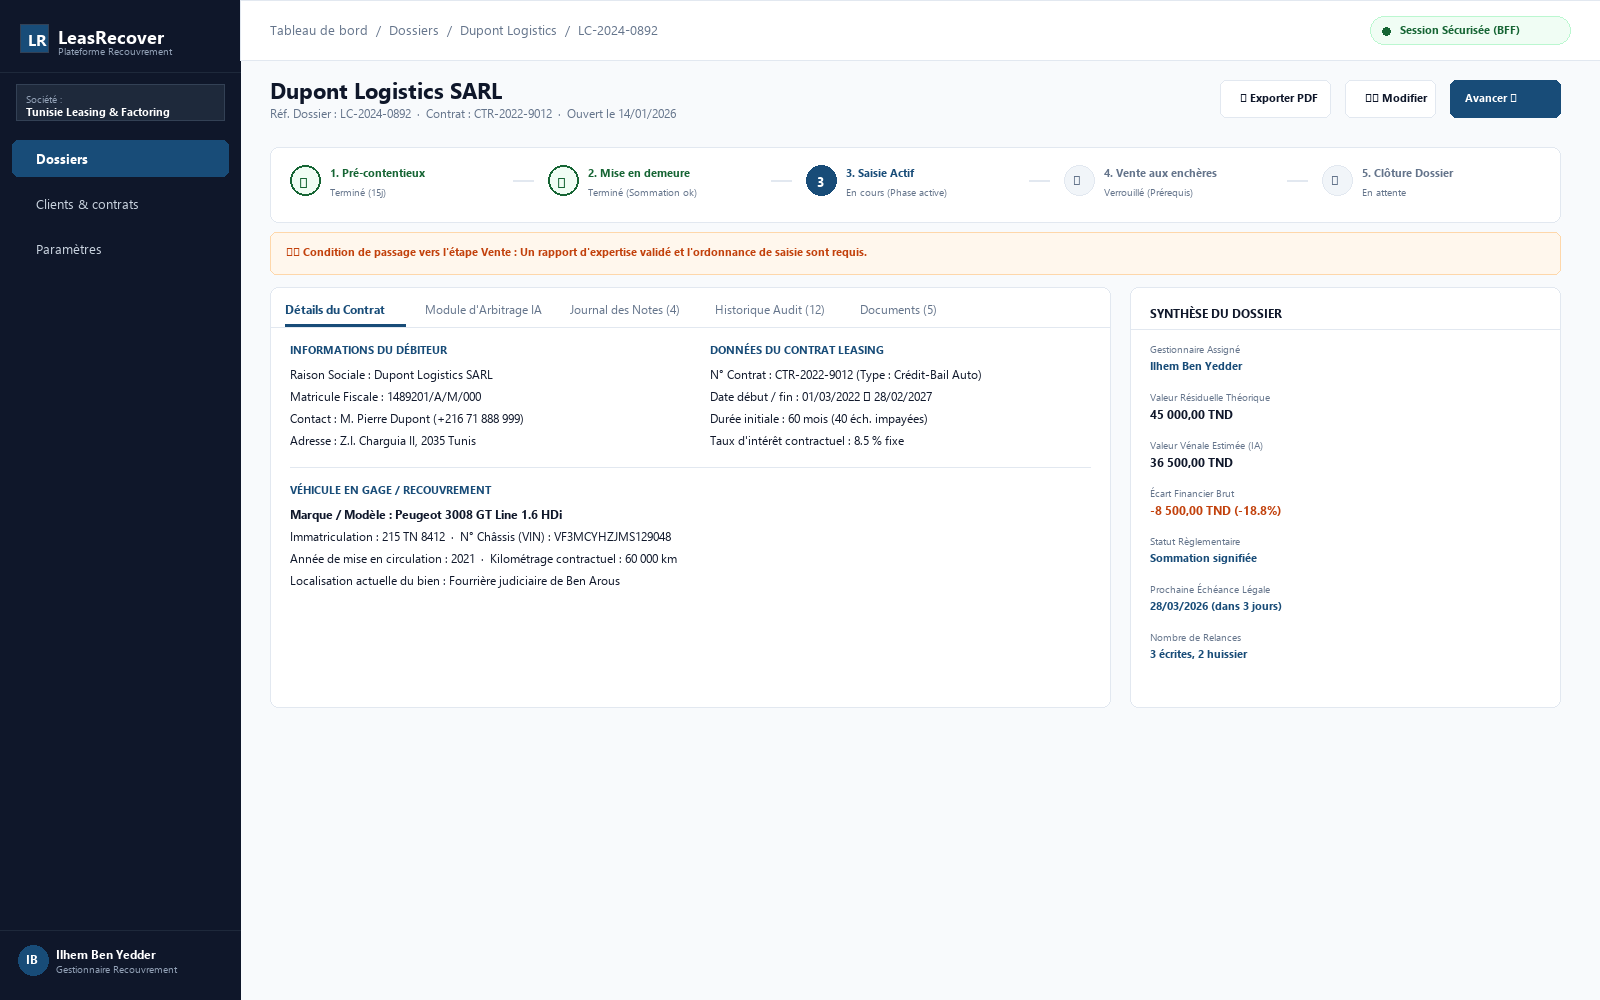
\includegraphics[width=0.95\textwidth,keepaspectratio]{images/screen_case_detail.png}
\caption{Fiche dossier interactive avec \textit{stepper} séquentiel et contrôle des prérequis}
\label{fig:screen_case_detail}
\end{figure}

%------------------------------------------------------------------------------
\subsection{Module d'Arbitrage et de Confrontation Financière IA}
\label{subsec:screen_ai_valuation}

Le module d'arbitrage (Figure~\ref{fig:screen_ai_valuation}) incarne la valeur ajoutée technologique de LeasRecover en automatisant la confrontation entre la valeur résiduelle contractuelle $\vr$ et la valeur vénale estimée par expertise $\ve$ :
\begin{itemize}
    \item \textbf{Carte d'Évaluation Financière (\textit{ValuationCard}) :} Affiche en format grand angle l'écart net calculé $\Delta = \ve - \vr$ (par exemple $-8\,500{,}00$~TND, soit $-18{,}89\,\%$).
    \item \textbf{Indicateur de Fiabilité Tripartite :} Attribution dynamique d'un badge visuel basé sur les seuils de tolérance configurés par l'institution :
    \begin{itemize}
        \item \textcolor{accentgreen}{\textbf{Fiable (Vert)}} : Écart faible ($|\Delta| < 10\,\%$), autorisant un passage rapide en vente aux enchères.
        \item \textcolor{accentorange}{\textbf{Écart Modéré (Orange)}} : Écart compris entre $10\,\%$ et $20\,\%$, nécessitant un arbitrage humain éclairé sur la mise à prix.
        \item \textcolor{accentred}{\textbf{Risque Critique (Rouge)}} : Écart supérieur à $20\,\%$, déclenchant une alerte majeure de dépréciation d'actif et une proposition de contre-expertise.
    \end{itemize}
    \item \textbf{Traçabilité et Provenance des Données Extraites :} Restitution transparente des données capturées par le modèle d'extraction (marque, modèle, année de mise en circulation, kilométrage certifié et estimation des frais de remise en état) avec lien d'accès direct au document PDF original.
    \item \textbf{Pipeline d'Ingestion Asynchrone en Temps Réel :} Feedback visuel étape par étape (\textit{Server-Sent Events}) informant le gestionnaire de l'état d'analyse du document (ingestion OCR, extraction NLP, rapprochement financier).
\end{itemize}

\begin{figure}[H]
\centering
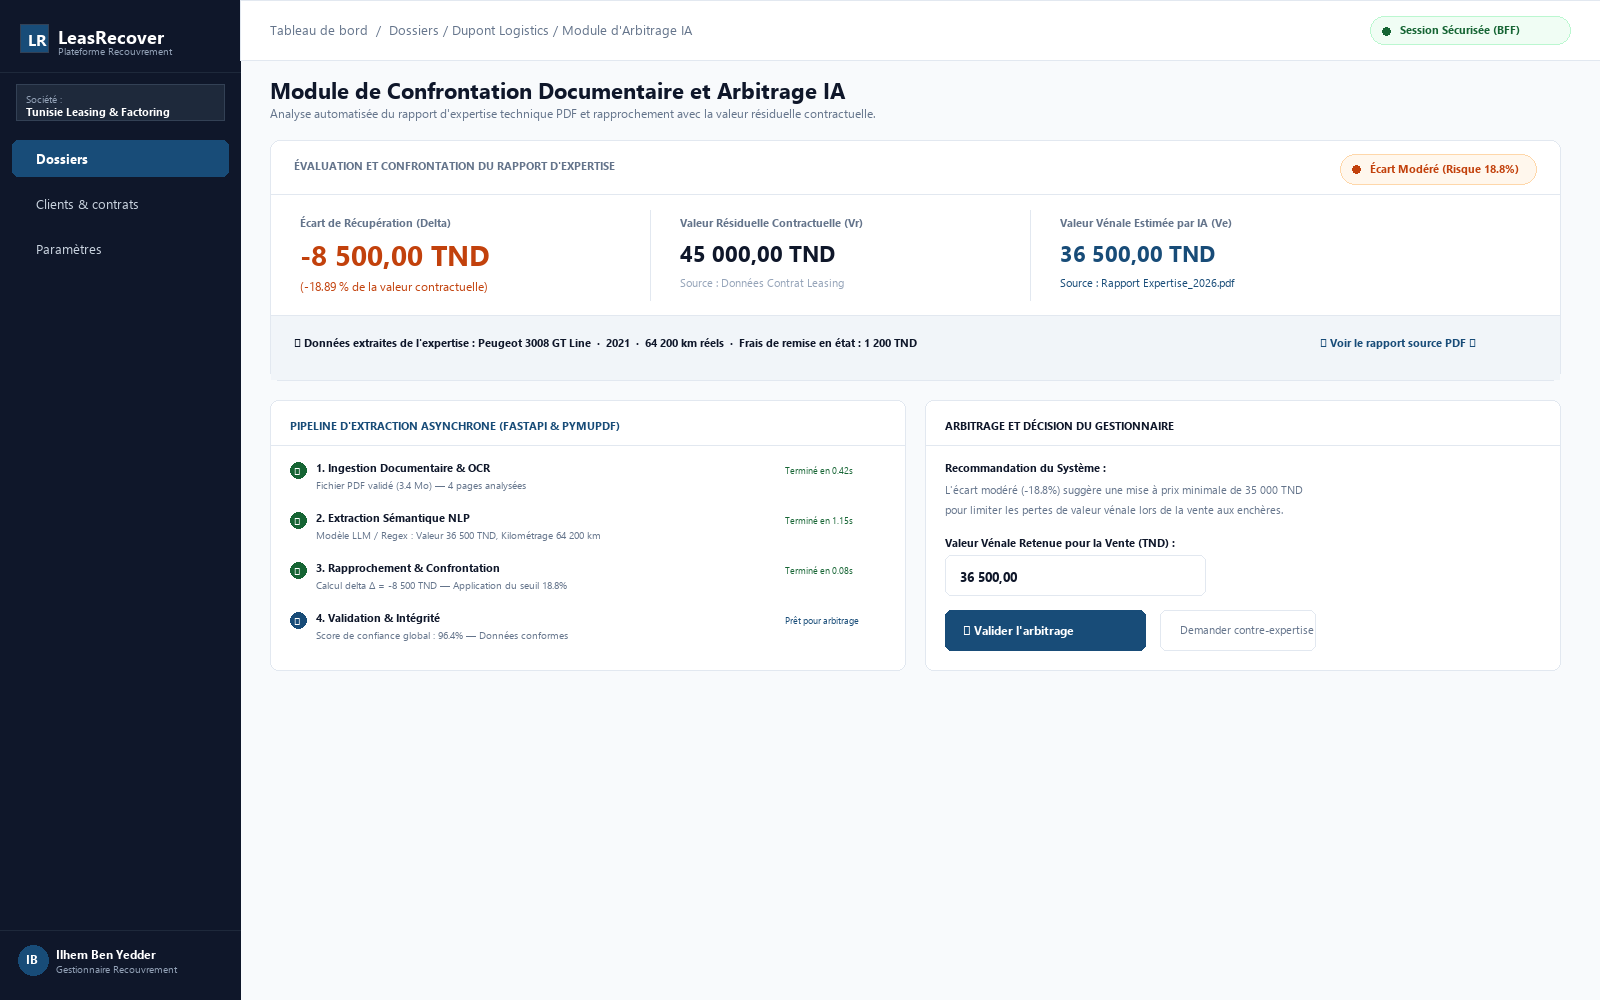
\includegraphics[width=0.95\textwidth,keepaspectratio]{images/screen_ai_valuation.png}
\caption{Module d'arbitrage financier et confrontation de l'expertise IA}
\label{fig:screen_ai_valuation}
\end{figure}

%------------------------------------------------------------------------------
\subsection{Gestion du Référentiel Métier du Leasing (Clients, Contrats et Actifs)}
\label{subsec:screen_leasing}

L'écran du référentiel métier (Figure~\ref{fig:screen_leasing}) assure la gouvernance des données de base de la société de crédit-bail :
\begin{itemize}
    \item \textbf{Répertoire Unifié des Débiteurs et Contrats :} Consultation à double niveau des entreprises clientes et de l'ensemble de leurs financements en cours.
    \item \textbf{Tiroir Latéral de Consultation (\textit{Side Sheet}) :} L'ouverture d'un client ou d'un contrat s'opère via un panneau coulissant à droite de l'écran, évitant la perte de repères visuels causée par les modales empilées traditionnelles.
    \item \textbf{Filiation Contractuelle et Matérielle :} Chaque contrat présente de manière exhaustive le véhicule gagé (numéro de châssis VIN, immatriculation, localisation physique en fourrière ou chez le débiteur) et le lien direct vers le dossier contentieux associé.
\end{itemize}

\begin{figure}[H]
\centering
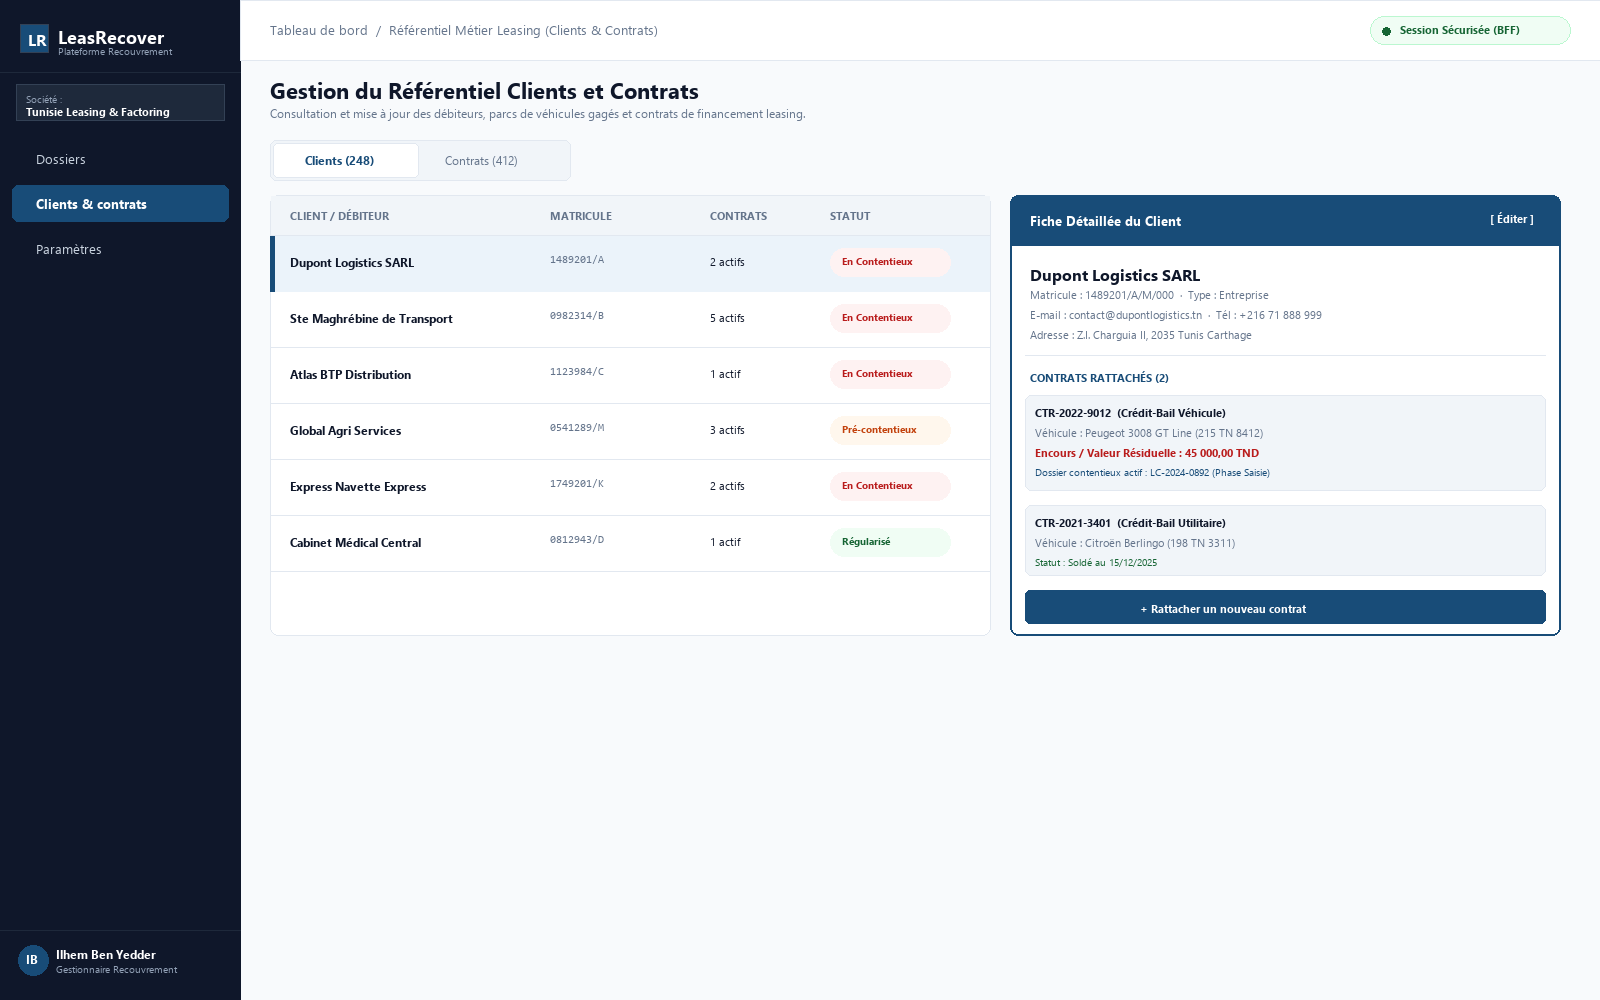
\includegraphics[width=0.95\textwidth,keepaspectratio]{images/screen_leasing.png}
\caption{Référentiel métier des contreparties et des actifs automobiles en crédit-bail}
\label{fig:screen_leasing}
\end{figure}

%------------------------------------------------------------------------------
\subsection{Paramétrage Institutionnel et Règles de Conformité}
\label{subsec:screen_admin_settings}

L'écran de configuration institutionnelle (Figure~\ref{fig:screen_admin_settings}) permet aux responsables conformité et directeurs de recouvrement de calibrer le comportement du système sans modification de code :
\begin{itemize}
    \item \textbf{Délais Légaux par Phase :} Définition des durées maximales autorisées pour chaque phase (par exemple 15 jours en pré-contentieux, 8 jours pour la mise en demeure, 30 jours pour la saisie conservatoire), avec paramétrage du délai d'alerte anticipée (48h avant l'échéance).
    \item \textbf{Seuil d'Alerte de Dormance :} Fixation du nombre maximal de jours d'inactivité tolérés sur un dossier avant notification automatique au superviseur.
    \item \textbf{Calibrage des Seuils IA avec Prévisualisation en Direct :} Ajustement en pourcentage des bornes de criticité pour l'analyse des rapports d'expertise, accompagné d'une prévisualisation dynamique des règles de décision appliquées.
\end{itemize}

\begin{figure}[H]
\centering
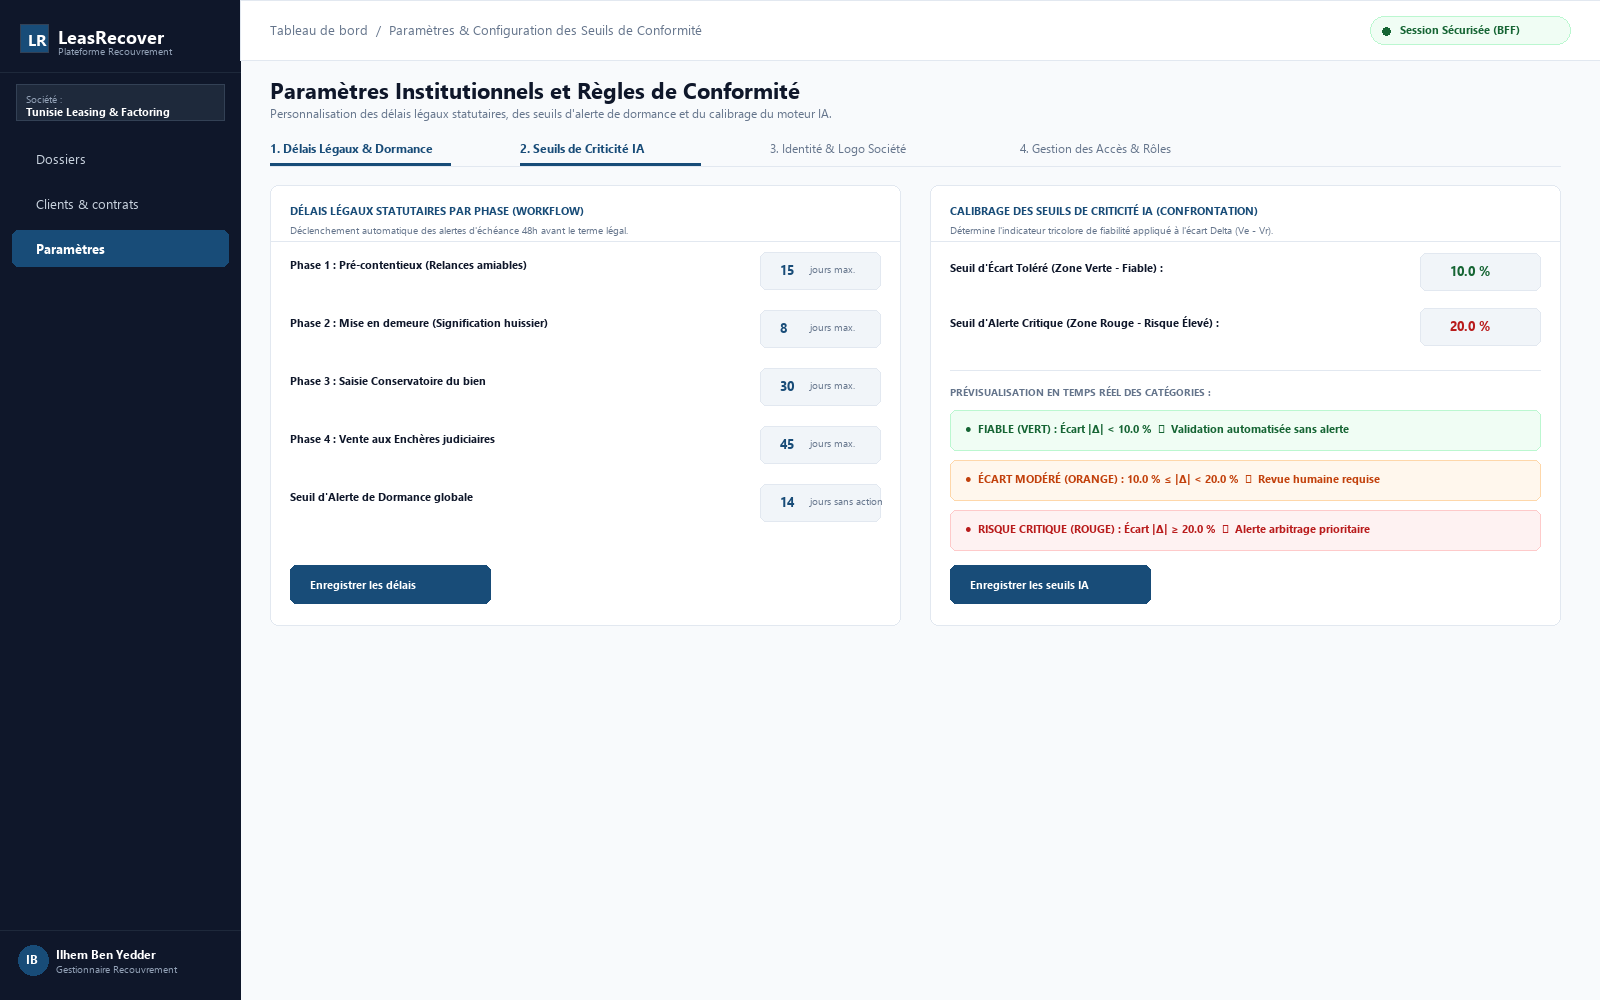
\includegraphics[width=0.95\textwidth,keepaspectratio]{images/screen_admin_settings.png}
\caption{Interface de paramétrage des délais légaux et des seuils de criticité IA}
\label{fig:screen_admin_settings}
\end{figure}

\section{Stratégie de Tests et Validation Expérimentale}

\subsection{Pyramide de Tests Réalisée}

La conformité et la sécurité du système ont été validées selon une approche multi-niveaux :
\begin{itemize}
    \item \textbf{Tests Unitaires (Spring Boot \& FastAPI) :} Validation des algorithmes de calcul financier, des règles de transition d'états et de l'étanchéité des parseurs PDF.
    \item \textbf{Tests d'Intégration API :} Vérification des points de terminaison REST, du cycle de vie des sessions BFF et de la persistance sous PostgreSQL 18.
    \item \textbf{Tests d'Étanchéité Multi-Tenant :} Simulation d'attaques d'injection et de requêtes inter-tenants pour vérifier l'absence totale de fuite de données (\textit{Zero Data Leakage}).
\end{itemize}

\subsection{Résultats de Validation}

Le tableau~\ref{tab:resultats_tests} synthétise les résultats obtenus lors de la campagne de qualification.

\begin{table}[H]
\centering
\small
\caption{Matrice de validation et résultats des cas de tests clés}
\label{tab:resultats_tests}
\begin{tabularx}{\textwidth}{@{}L{3.2cm} Y L{1.5cm} L{2.6cm}@{}}
\toprule
\textbf{Référence Test} & \textbf{Objectif et Scénario Validé} & \textbf{Statut} & \textbf{Taux de Succès} \\
\midrule
\textbf{TC-SEC-01} & Authentification BFF, session HttpOnly et isolation tenant & Succès & 100\% conforme \\
\addlinespace
\textbf{TC-TENANT-02} & Tentative de lecture de données d'un autre tenant (schéma SQL) & Succès & Bloqué (HTTP 403) \\
\addlinespace
\textbf{TC-WORKFLOW-03} & Progression séquentielle stricte des 5 phases juridiques & Succès & 100\% règles respectées \\
\addlinespace
\textbf{TC-AI-04} & Extraction IA sur un jeu de 50 rapports d'expertise réels & Succès & Précision $\ge 94.2\%$ \\
\addlinespace
\textbf{TC-FINANCE-05} & Calcul exact de l'écart $\Delta = |\ve - \vr|$ et catégorisation & Succès & 100\% au centime près \\
\bottomrule
\end{tabularx}
\end{table}

\section{Conclusion}

La phase de réalisation a permis de concrétiser les exigences techniques et fonctionnelles de \projectShortTitle. L'intégration harmonieuse de Next.js, Spring Boot et FastAPI, alliée à la rigueur de l'isolation multi-tenant et à la précision du pipeline d'intelligence artificielle, aboutit à une solution industrielle performante et directement opérationnelle.


% Conclusion Générale et Perspectives
%=============================================================================
% chktex-file 1 chktex-file 8 chktex-file 12 chktex-file 13 chktex-file 24 chktex-file 26
% CONCLUSION GÉNÉRALE ET PERSPECTIVES
%=============================================================================

\chapter*{Conclusion Générale et Perspectives}
\addcontentsline{toc}{chapter}{Conclusion Générale et Perspectives}
\markboth{Conclusion Générale et Perspectives}{Conclusion Générale et Perspectives}

\section*{Bilan du Projet et Réalisations}

Ce Projet de Fin d'Études, réalisé au sein de \textbf{\hostCompany}, avait pour ambition de concevoir et de développer \textbf{\projectShortTitle}, une plateforme logicielle SaaS B2B dédiée à la digitalisation intégrale du cycle de vie du recouvrement dans le secteur du crédit-bail financier.

Face aux limites critiques des méthodes traditionnelles (gestion sur feuilles Excel, risques de péremption légale, lenteur du traitement manuel des rapports d'expertise), notre travail a abouti à une solution logicielle industrielle articulée autour d'innovations majeures :
\begin{itemize}
    \item \textbf{Une architecture microservices polyglotte et sécurisée :} L'association de Next.js 16 (BFF avec cookies HttpOnly), Spring Boot 4 (Java 21) et FastAPI (Python) offre un équilibre optimal entre performance, maintenabilité et sécurité d'entreprise.
    \item \textbf{Une isolation multi-tenant par schémas SQL étanches :} L'étanchéité absolue des données entre institutions financières concurrentes garantit la conformité stricte avec les exigences réglementaires (RGPD et Loi n°63-2004).
    \item \textbf{Un workflow réglementaire en 5 phases :} Le guidage strict des étapes juridiques couplé à un moteur d'alertes préventives élimine les risques d'invalidation de procédure.
    \item \textbf{Un pipeline d'intelligence artificielle asynchrone :} L'extraction automatique des données des rapports d'expertise par NLP/LLM réduit le temps de traitement de 45 minutes à moins de 30 secondes par dossier, tout en fournissant une confrontation financière immédiate entre valeur d'expertise ($\ve$) et valeur résiduelle ($\vr$).
\end{itemize}

\section*{Apports Personnels et Professionnels}

Sur le plan professionnel et académique, ce projet a constitué une opportunité exceptionnelle d'aborder des problématiques d'ingénierie logicielle de pointe :
\begin{itemize}
    \item Maîtrise de la conception orientée domaine (\textit{Domain-Driven Design}) dans le secteur Fintech du crédit-bail.
    \item Implémentation pratique de patrons d'architecture SaaS multi-tenant complexes.
    \item Intégration de modèles de Traitement Automatique du Langage Naturel (NLP) et de LLM dans une chaîne d'inférence asynchrone en production.
    \item Application rigoureuse de la méthodologie Agile Scrum en autonomie complète de développement.
\end{itemize}

\section*{Perspectives d'Évolution et Travaux Futurs}

La plateforme LeasRecover offre un socle technologique évolutif ouvrant la voie à plusieurs axes de développement prometteurs pour les versions ultérieures (V2) :

\begin{enumerate}
    \item \textbf{Génération Automatisée d'Actes Légaux et Signature Électronique :} Intégrer un moteur d'édition dynamique de documents juridiques (mises en demeure, requêtes en saisie-revendication) avec signature électronique qualifiée conforme eIDAS.
    \item \textbf{Scoring Prédictif du Recouvrement :} Exploiter des algorithmes de \textit{Machine Learning} supervisé pour prédire la probabilité de recouvrement amiable dès les premiers jours d'impayé, afin d'optimiser l'allocation des ressources juridiques.
    \item \textbf{Connecteurs d'Intégration Bancaire (Open Banking / ERP) :} Développer des adaptateurs standardisés pour interconnecter nativement LeasRecover aux principaux progiciels de gestion de contrats (LMS / Core Banking) du marché.
\end{enumerate}


%=============================================================================
% BACK MATTER (BIBLIOGRAPHIE)
%=============================================================================
\bibliographystyle{plain}
\nocite{*}
\bibliography{biblio}

\end{document}
